\chapter{Dispersed phase simulations in BIMER}
	\label{ch9:BIMER_lagrangian}

\section{Introduction}

The previous chapter has reported the resolved atomization simulations performed through one multipoint injector of the BIMER configuration. The lagrangian injector learning process was applied to get a in-plane, spatially distributed spray. This spray conforms a lagrangian injector that is used in this chapter to initialize the liquid phase dispersed-phase simulations. The dense core was also characterized: these information can be used in this chapter to impose an actuator with the ALM method that perturbs the gaseous phase similarly to a jet dense column. Due to rotational symmetry in the multipoint stage, the obtained SLI and actuator can be extrapolated to the remaining multipoint holes to perform liquid injection and gaseous phase perturbation in the full configuration. This chapter reports the results of \hl{one (two?)} dispersed-phase simulation\hl{(s)} of BIMER with the SLI methodology.

In first place, the computational setup is explained in $\S$\ref{ch9:sec_computations_setup}. The multipoint injection is briefly detailed here, while the pilot injection performed with the LISA injection model is thoroughly explained. Then, available experimental results for this configuration and the operating point chosen, which can be used for computational validation, obtained by \citeColor[renaud_high-speed_2015] are summarized in $\S$\ref{ch9:sec_expe_results_LGS_BIMER}. The SLI flowchart, which was generally detailed in Figure \ref{fig:SLI_graphic_description} for a JICF, is extended to BIMER in $\S$\ref{sec:ch9_BIMER_SLI_flowchart}. Next, the SLI used for lagrangian injector and the effect of the proposed ALM in the gaseous field are reported in $\S$\ref{sec:ch9_BIMER_BCs_for_phases}. Finally, the results from \hl{one (two)}  simulation\hl{(s)} are reported and discussed in $\S$\hl{\textbf{XX}}. \hl{It is shown that ...}





\section{Computational setup}
\label{ch9:sec_computations_setup}


For performing dispersed phase simulations, the operating point defined in Table \ref{tab:liquid_operating_point_Renaud} is simulated. The staging factor is $\alpha = 15$, meaning that $15 \%$ of the total liquid flow rate is injected through the pilot stage and the remaining liquid through the multipoint. For total flow rate of $\dot{m}_l = 1.64$ g s$^{-1}$, the take-off stage injects a mass flow rate of $\dot{m}_{l,takeoff}$ = 1.39 g s$^{-1}$ (hence $0.139$ g s$^{-1}$, corresponding to $Q_l = 185.3$ mm$^3$s$^{-1}$,  per injector), and a mass flow rate of $\dot{m}_{l,p} = 0.25$ g s$^{-1}$ is introduced through the pilot stage. The global equivalence ratio of this operating point is $\phi_g = 0.6$.

\subsubsection*{Evaporation}

Due to the high gas ambient temperature inside BIMER combustion chamber ($T_g = 433$ K while $T_l = 293$ K, see Table \ref{tab:liquid_operating_point_Renaud}), evaporation of lagrangian droplets should be considered. For assessing this influence, the evaporation model of \citeColor[spalding_combustion_1954] is used in one simulation, which is compared to two other simulations where mass and heat transfer are not taken into account. Details on the hypothesis and implementation of this evaporation model in YALES2 can be found in \citeColor[domingo-alvarez_high-pressure_2019].

%\begin{table}[!h]
%\centering
%\caption{Operating point to perform gaseous and two-phase simulations tested by \citeColor[renaud_high-speed_2015]}
%\begin{tabular}{|c|c|c|c|}
%\hline
%\multicolumn{4}{|c|}{\textbf{Air properties}} \\
%\hline
%$\dot{m}_g$ [g s$^{-1}$] & $T_g$ [K] & $\rho_g$ [kg m$^{-3}$]  & $\mu_g$ [Pa s]  \\
%\hline
%43.1 & 433 & 0.816382 & $2.3911 \cdot 10^{-5}$ \\
%\hline
%\hline
%\multicolumn{4}{|c|}{\textbf{Liquid properties}} \\
%\hline
%$\dot{m}_l$ [g s$^{-1}$] & $\rho_l$ [kg m$^{-3}]$   & $\mu_l$ [Pa s]   & $\sigma$ [N m$^{-1}$]   \\
%\hline
%1.64 & 750 & $1.36 \cdot 10^{-3}$ & $25.35 \cdot 10^{-3}$ \\
%\hline
%\hline
%\multicolumn{4}{|c|}{\textbf{Burner staging}} \\
%\hline
%$\alpha$ [$\%$] &  $\dot{m}_{l,p}$ [g s$^{-1}$] & $\dot{m}_{l,t}$ [g s$^{-1}$] & $\phi_g$ [-]\\
%\hline
%15 & 0.25 & 1.39 & 0.6 \\
%\hline
%\end{tabular}
%\label{tab:liquid_operating_point_Renaud}
%\end{table}

\clearpage


\begin{table}[!h]
\centering
\caption{Operating point to perform gaseous and two-phase simulations tested by \citeColor[renaud_high-speed_2015]}
\begin{tabular}{cccc}
\thickhline
\multicolumn{4}{c}{\textbf{Air properties}} \\
\hline
$\dot{m}_g$ [g s$^{-1}$] & $T_g$ [K] & $\rho_g$ [kg m$^{-3}$]  & $\mu_g$ [Pa s]  \\
\hline
43.1 & 433 & 0.82 & $2.4 \cdot 10^{-5}$ \\[0.075in] %0.816382 & $2.3911 \cdot 10^{-5}$ \\[0.075in]
%%\bottomrule
%\\[0.1in]
%%\vspace*{0.1in}
\thickhline
\multicolumn{4}{c}{\textbf{Liquid properties}} \\
\hline
$\sigma$ [N m$^{-1}$] & $T_l$ [K] & $\rho_l$ [kg m$^{-3}]$   & $\mu_l$ [Pa s]    \\
\hline
$25 \cdot 10^{-3}$ & 293 & 750 & $1.36 \cdot 10^{-3}$   \\[0.075in] %25.35 
\thickhline
\multicolumn{4}{c}{\textbf{Burner staging}} \\
\hline
$\alpha$ [$\%$] &  $\dot{m}_{l,pilot}$ [g s$^{-1}$] & $\dot{m}_{l,takeoff}$ [g s$^{-1}$] & $\phi_g$ [-]\\
\hline
15 & 0.25 & 1.39 & 0.6 \\
\thickhline
\end{tabular}
\label{tab:liquid_operating_point_Renaud}
\end{table}


%\begin{table}[!h]
%\centering
%\caption{Operating point to perform gaseous and two-phase simulations tested by \citeColor[renaud_high-speed_2015]}
%\begin{tabular}{cccc}
%\thickhline
%\multicolumn{4}{c}{\textbf{Air properties}} \\
%\hline
%$\dot{m}_g$ [g s$^{-1}$] & $T_g$ [K] & $\rho_g$ [kg m$^{-3}$]  & $\mu_g$ [Pa s]  \\
%\hline
%43.1 & 433 & 0.82 & $2.4 \cdot 10^{-5}$ \\[0.075in] %0.816382 & $2.3911 \cdot 10^{-5}$ \\[0.075in]
%%%\bottomrule
%%\\[0.1in]
%%%\vspace*{0.1in}
%\thickhline
%\multicolumn{5}{c}{\textbf{Liquid properties}} \\
%\hline
%$\dot{m}_l$ [g s$^{-1}$] & $\rho_l$ [kg m$^{-3}]$   & $\mu_l$ [Pa s]   & $\sigma$ [N m$^{-1}$]  \\
%\hline
%1.64 & 750 & $1.36 \cdot 10^{-3}$ & $25 \cdot 10^{-3}$ \\[0.075in] %25.35 
%\thickhline
%\multicolumn{4}{c}{\textbf{Burner staging}} \\
%\hline
%$\alpha$ [$\%$] &  $\dot{m}_{l,pilot}$ [g s$^{-1}$] & $\dot{m}_{l,takeoff}$ [g s$^{-1}$] & $\phi_g$ [-]\\
%\hline
%15 & 0.25 & 1.39 & 0.6 \\
%\thickhline
%\end{tabular}
%\label{tab:liquid_operating_point_Renaud}
%\end{table}








%\begin{table}[!h]
%\centering
%\caption{Operating point to perform gaseous and two-phase simulations tested by \citeColor[renaud_high-speed_2015]}
%\begin{tabular}{cccc}
%\thickhline
%\multicolumn{4}{c}{\textbf{Air properties}} \\
%\thickhline
%$\dot{m}_g$ [g s$^{-1}$] & $T_g$ [K] & $\rho_g$ [kg m$^{-3}$]  & $\mu_g$ [Pa s]  \\
%\hline
%43.1 & 433 & 0.816382 & $2.3911 \cdot 10^{-5}$ \\
%\end{tabular} \\
%\medskip
%\begin{tabular}{cccc}
%\thickhline
%\multicolumn{4}{c}{\textbf{Liquid properties}} \\
%\hline
%$\dot{m}_l$ [g s$^{-1}$] & $\rho_l$ [kg m$^{-3}]$   & $\mu_l$ [Pa s]   & $\sigma$ [N m$^{-1}$]   \\
%\hline
%1.64 & 750 & $1.36 \cdot 10^{-3}$ & $25.35 \cdot 10^{-3}$ \\
%\end{tabular} \\
%\medskip
%\begin{tabular}{cccc}
%\thickhline
%\multicolumn{4}{c}{\textbf{Burner staging}} \\
%\hline
%$\alpha$ [$\%$] &  $\dot{m}_{l,p}$ [g s$^{-1}$] & $\dot{m}_{l,t}$ [g s$^{-1}$] & $\phi_g$ [-]\\
%\hline
%15 & 0.25 & 1.39 & 0.6 \\
%\hline
%\end{tabular}
%\label{tab:liquid_operating_point_Renaud}
%\end{table}





\section{Experimental results from literature}
\label{ch9:sec_expe_results_LGS_BIMER}

The BIMER operating point tested in this chapter to test the SLI methodology has been chosen since it presents non-reactive experimental results that can be used for validation. These ones, shown in the PhD thesis of \citeColor[renaud_high-speed_2015], consist of the qualitative maps of SMD and axial velocity shown in Figure \ref{fig:maps_BIMER_renaud_expe_results}. From the SMD map at the left, a global SMD in the disclosed region is 16.58 $\mu$m. Further qualitative experimental results on non-reactive conditions are not available from literature, and hence a qualitative validation is not possible to this date.

%\begin{figure}[h!]
%\flushleft
%\begin{subfigure}[b]{0.3\textwidth}
%	\centering
%   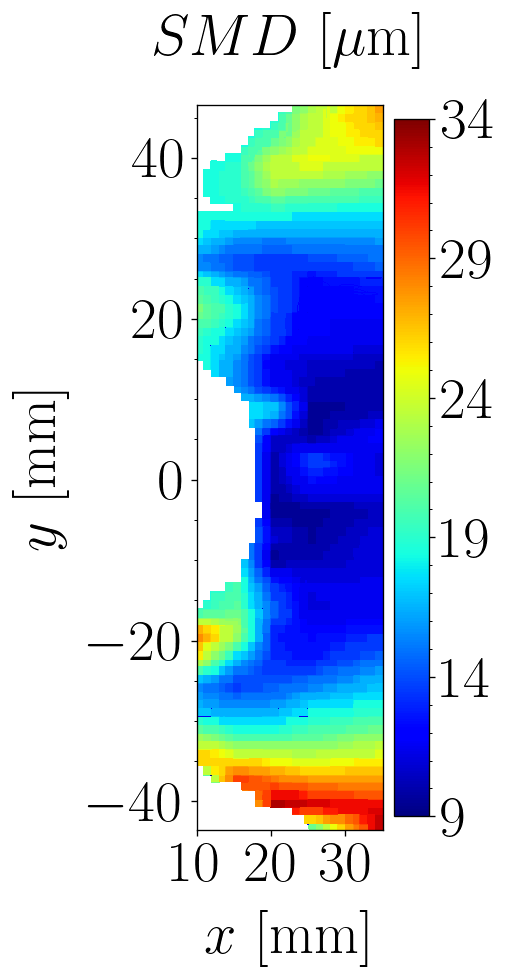
\includegraphics[scale=0.4]{./part3_applications/figures_ch9_lagrangian/expe_maps/SMD_map.png}
%   %\caption{Low Weber number operating point.}
%   %\label{} 
%\end{subfigure}
%\hspace*{0.1in}
%\begin{subfigure}[b]{0.3\textwidth}
%	\centering
%   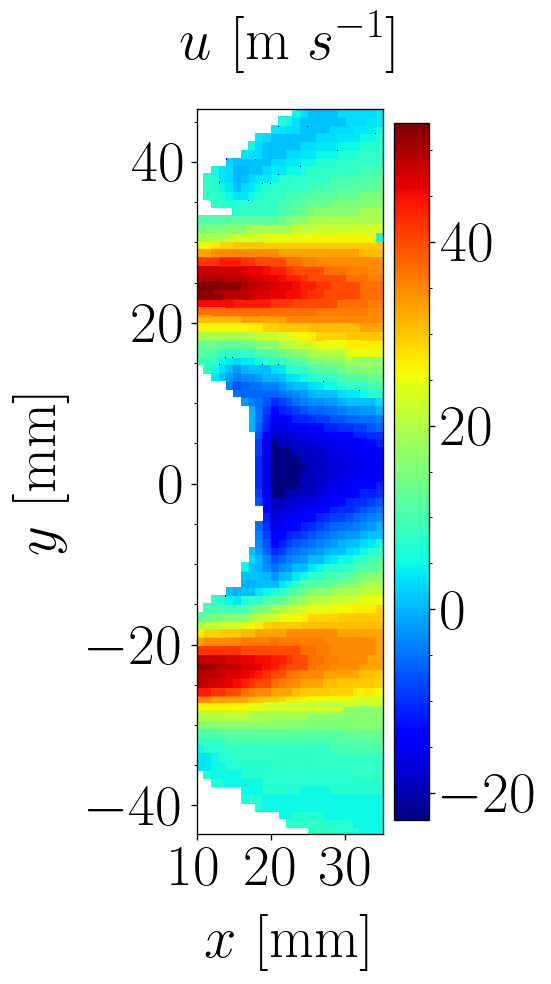
\includegraphics[scale=0.4]{./part3_applications/figures_ch9_lagrangian/expe_maps/u_axial_map.png}
%   %\caption{Low Weber number operating point.}
%   %\label{} 
%\end{subfigure}
%\hspace*{0.1in}
%\begin{subfigure}[b]{0.3\textwidth}
%	\centering
%   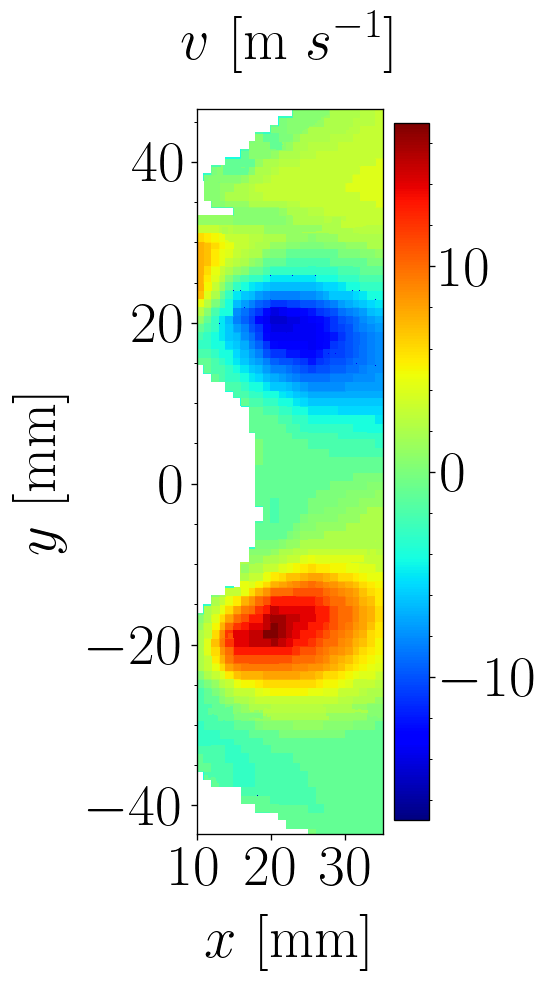
\includegraphics[scale=0.4]{./part3_applications/figures_ch9_lagrangian/expe_maps/u_vertical_map.png}
%   %\caption{Low Weber number operating point.}
%   %\label{} 
%\end{subfigure}
%\caption{Experimental maps for for $SMD$, axial velocity $u$ and vertical velocity $v$ from \citeColor[renaud_high-speed_2015]}
%\label{fig:maps_BIMER_renaud_expe_results}
%\end{figure}


\begin{figure}[h!]
\flushleft
\begin{subfigure}[b]{0.45\textwidth}
	\flushright
   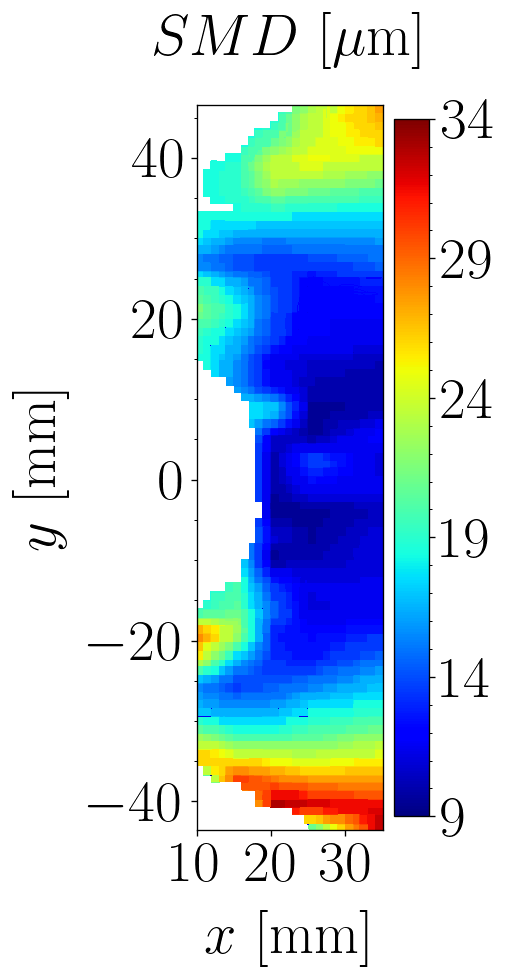
\includegraphics[scale=0.3]{./part3_applications/figures_ch9_lagrangian/expe_maps/SMD_map.png}
   %\caption{Low Weber number operating point.}
   %\label{} 
\end{subfigure}
\hspace*{0.05in}
\begin{subfigure}[b]{0.45\textwidth}
	\flushleft
   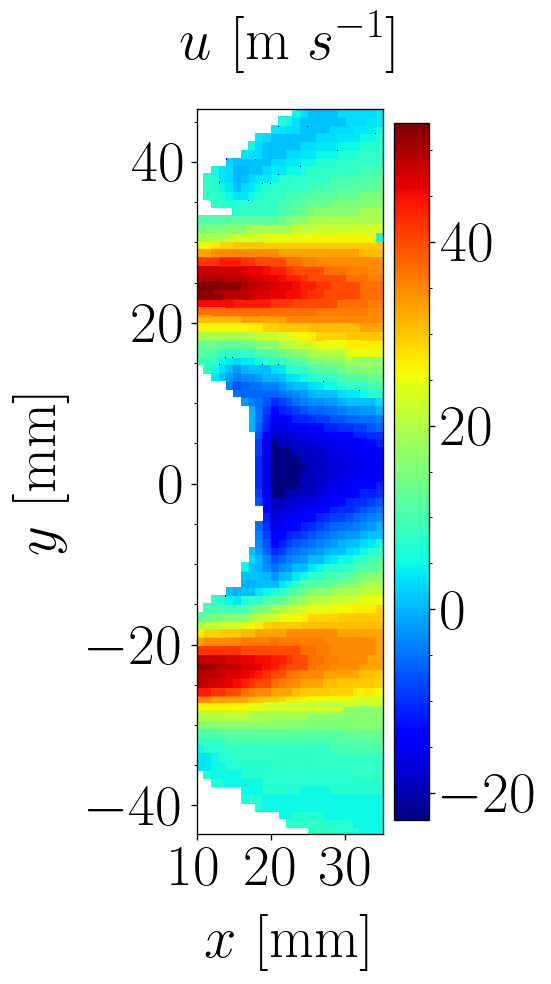
\includegraphics[scale=0.3]{./part3_applications/figures_ch9_lagrangian/expe_maps/u_axial_map.png}
   %\caption{Low Weber number operating point.}
   %\label{} 
\end{subfigure}
\caption{Experimental maps for for $SMD$ and axial velocity $u$ from \citeColor[renaud_high-speed_2015]}
\label{fig:maps_BIMER_renaud_expe_results}
\end{figure}


%\begin{figure}[h!]
%\flushleft
%\begin{subfigure}[b]{0.3\textwidth}
%	\centering
%   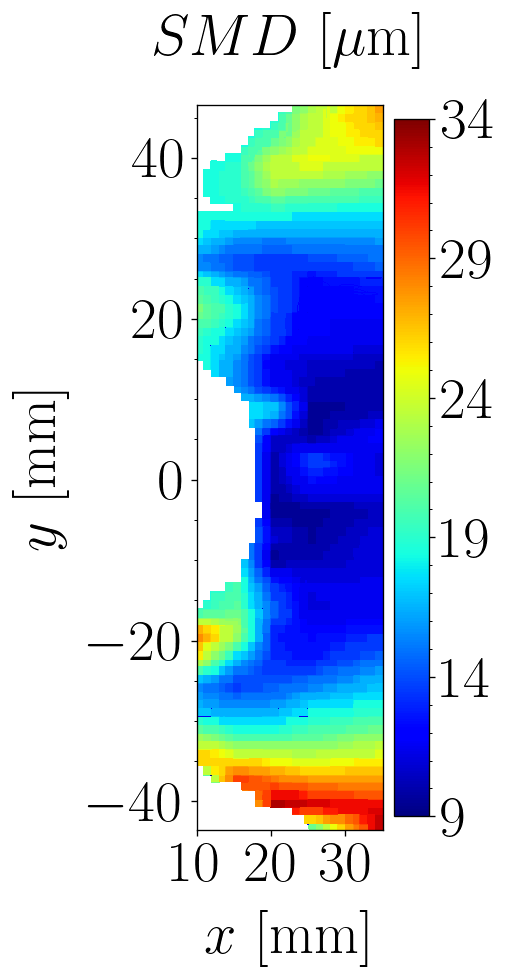
\includegraphics[scale=0.3]{./part3_applications/figures_ch9_lagrangian/expe_maps/SMD_map.png}
%   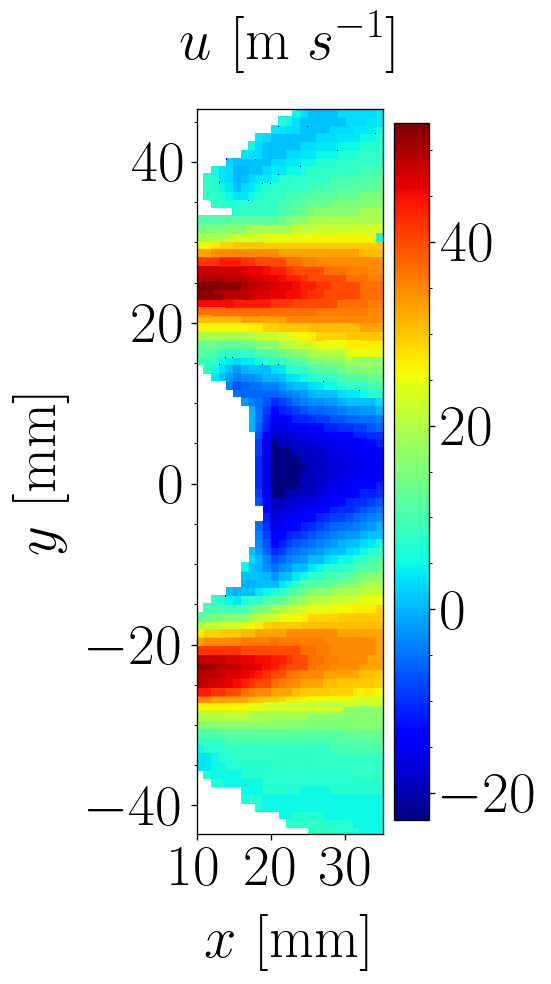
\includegraphics[scale=0.3]{./part3_applications/figures_ch9_lagrangian/expe_maps/u_axial_map.png}
%\caption{Experimental maps for for $SMD$ and axial velocity $u$ from \citeColor[renaud_high-speed_2015]}
%\label{fig:maps_BIMER_renaud_expe_results}
%\end{figure}


\section{Boundary condition for liquid phase}
\label{sec:ch9_BIMER_BCs_for_liquid_phase}


\subsection{Multipoint stage injection}

For the multipoint stage, the SLI obtained from the resolved atomization simulations in Chapter \ref{ch8:bimer_resolved_atomization} are used. Since the objective of this simulation is to prove that SLI can be used to initialise dispersed-phase computations in a full multipoint injector, only the SLI obtained from the fine simulation with $\Delta x_\mathrm{min} = 10~\mu$m at the location $x_c = 2$ mm is used. This injector is chosen since 1) it has been obtained with the finest interface resolution simulated and 2) it has been obtained at an axial location along the crossflow direction $x_c$ where all the global spray mean magnitudes (SMD, velocities, deformation parameters) are converged with axial distance (see $\S$\ref{sec:ch8_BIMER_spray_char}). This SLI is shown in Figure \ref{fig:injectors_sli_BIMER_DX10_xD06p67}: these maps, without convergence-driven discretization, are injected as shown in the dispersed phase simulation. The flux spatial distribution in the SLI is scaled so that the total mass flow rate injected in one multipoint hole is equal to the actual mass flow rate injected in the experimental configuration. Injected velocities are volume-weighted and RMS following a gaussian $r$ velocity law. For secondary atomization, all the three models has been tested but none of them has shown to actually predict any breakup event throughout the simulations: the injected droplets from both multipoint and pilot stages are considered to be in equilibrium by the breakup models, and hence particles are not broken by secondary atomization. %The relevant injection parameters for the multipoint stage are summarized in Table  \ref{tab:BIMER_SLI_fixed_model_parameters}.

%\begin{table}[!h]
%\centering
%\caption{Fixed SLI model parameters for dispersed-phase simulations of the take-off stage in BIMER}
%\begin{tabular}{ccc}
%\thickhline
% \multirow{2}{*}{ \begin{tabular}{c} \textbf{Resolved} \\ \textbf{simulation} \end{tabular}}    &  \multirow{2}{*}{  \begin{tabular}{c} $x_{c,\mathrm{inj}}$  \\ $\left[ \mathrm{mm} \right]$ \end{tabular}} &   \multirow{2}{*}{ \begin{tabular}{c} $\textbf{r}$ \\ \textbf{law} \end{tabular}} \\
% & &  \\
%\thickhline
%DX10 & 2 & Gaussian  \\
%\thickhline
%\end{tabular}
%\label{tab:BIMER_SLI_fixed_model_parameters}
%\end{table}


%\begin{table}[!h]
%\centering
%\caption{Fixed SLI model parameters for dispersed-phase simulations of the take-off stage in BIMER}
%\begin{tabular}{cccccc}
%\thickhline
% \multirow{2}{*}{ \begin{tabular}{c} \textbf{Resolved} \\ \textbf{simulation} \end{tabular}}    &  \multirow{2}{*}{  \begin{tabular}{c} $x_{c,\mathrm{inj}}$  \\ $\left[ \mathrm{mm} \right]$ \end{tabular}} &   \multirow{2}{*}{ \begin{tabular}{c} $\textbf{r}$ \\ \textbf{law} \end{tabular}} & \multirow{2}{*}{ \begin{tabular}{c} \textbf{Atomization} \\ \textbf{model} \end{tabular}} &    \multirow{2}{*}{ $K_1$} & \multirow{2}{*}{ $K_2$}\\
% & & & & &  \\
%\thickhline
%DX10 & 2 & Gaussian & Goro  & ? & ? \\
%\thickhline
%\end{tabular}
%\label{tab:BIMER_SLI_fixed_model_parameters}
%\end{table}


For performing injection in the 10 multipoint holes, the SLI from the single liquid injector simulated are replicated in the remaining liquid injectors. For it, the injectors location are translated and the vectorial magnitudes (crossflow normal direction, velocities) are rotated so that the crossflow local direction stays identical in all multipoint holes. Each single injector will deliver a mass flow rate of $\dot{m}_{l,t} = 0.139$ g s$^{-1}$ (equivalent to a flow rate of $Q_l = 185.3$ mm$^3$ s$^{-1}$), hence making a total liquid flux injected of $\dot{m}_{l,t} = 1.39$ g s$^{-1}$ for the take-off phase as indicated in Table \ref{tab:liquid_operating_point_Renaud}. A schematic view of injectors through which lagrangian droplets are injected can be seen in Figure \ref{fig:BIMER_LGS_spray_establishment}.

%These injectors were, however, obtained from the simulations of one single injector. In order to initialise the rest of multipoint injection holes (for a total of 10 in BIMER, see Figure \textbf{Figure??}), new numerical injectors need to be defined in each hole by making a revolution of the available ones. This revolution is possible due to the radial of BIMER in terms of injectors location (which are equally spaced to a distance of 25 mm from the center with a radial difference of 36 $\degree$) and the multipoint vane locations: each injection hole is located at the same location between two vanes, hence seeing the same incoming air (see Figure \textbf{Figure??}).

%\begin{figure}[h!]
%	\centering	\includeinkscape[inkscapelatex=false,scale=0.5]{./part3_applications/figures_ch9_lagrangian/multipoint_injection_planes_view}
%	\caption{View of BIMER take-off stage showing three different injection locations}	\label{fig:BIMER_multipoint_injection_planes_view}
%\end{figure}
%




\subsection{Pilot stage injection}

The operating point simulated injects fuel through both a take-off stage (which has been modelled with the SLI) and a pilot stage. Since pilot stage has not been simulated with the methodology developed in this thesis, another approach must be employed. Given that the pilot of BIMER injects fuel following a hollow cone configuration, the LISA model introduced in $\S$\ref{subsec:ch3_hollow_cone_spray} will be used \citepColor[guedot_developpement_2015].   The input parameters for the LISA model to inject a hollow cone spray are summarized in Table \ref{tab:LISA_model_parameters}. For the mean opening angle, a value $\theta_s = 30 \degree$ is taken from experiments \citepColor[renaud_high-speed_2015]. Regarding the droplet's diameter, previous studies using lagrangian approaches on the same configuration have introduced directly droplets size distributions extracted from experimental data \citepColor[mesquita_large_2018]. In this case, since for the operating condition simulated there is not experimental size distributions available, droplets injected will have a constant diameter given by the following experimental correlation \citepColor[lefebvre_atomization_2017]:

\begin{equation}
SMD = 2.25 \left( \sigma \dot{m}_f \mu_l \right)^{0.25} \rho_g^{-0.25}  \Delta P^{-0.5}
\end{equation}

where $\Delta P = 2.6$ MPa is the pressure drop in the pilot nozzle \citeColor[renaud_high-speed_2015]. Applying the previous correlation with the magnitudes given in Table \ref{tab:liquid_operating_point_Renaud} results in a diameter $SMD = 15~\mu$m imposed constant to the pilot cones particles. As for the multipoint injection, secondary atomization models were applied to  particles introduced by the pilot stage without triggering any breakup effects. Hence, pilot droplets with a diameter of $15~\mu$m will not be reduced into smaller children particles due to secondary breakup, and will be solely transported for cases without evaporation. 

 %this correlation provides a SMD of $15 \mu m$ (\textbf{CHECK THIS}).

% dP value is tiven in Renaud p. 24, or 46 PDF

\begin{table}[!h]
\centering
\caption{LISA model setup for pilot injection}
\begin{tabular}{ccc}
\thickhline
\textbf{Parameter} & \textbf{Units} &  \textbf{Value} \\
\thickhline
Mass flow rate $\dot{m}$ & g s$^{-1}$ & 0.25 \\
%\hline
Injector radius $R_0$ & mm & 0.125 \\
%\hline
Mean angle $\overline{\theta}_s$ & $\degree$ & 30  \\
SMD & $\mu$m & 15 \\
\thickhline
\end{tabular}
\label{tab:LISA_model_parameters}
\end{table}




\section{Boundary condition for gaseous phase}
\label{sec:ch9_BIMER_BCs_for_gaseous_phase}

The perturbation effect of the liquid dense core, which is be directly accounted for by the lagrangian droplets, can also be modelled in BIMER. In this case, the direct prescription of a perturbed gaseous inlet in a reduced domain as described in $\S$\ref{subsec:ch6_jicf_lgs_gaseous_inlet_prescription} is not performed due to the complex geometrical features of the swirl injector. Therefore, only the ALM methodology ($\S$\ref{sec:ch4_dense_core_modelling}) is applied for this purpose. In a first step, the input parameters to the model are taken from the results of the resolved atomization simulation DX10: dense core topology from the results shown in Figure \ref{fig:BIMER_DC_mean_parameters_scatterplots} and net force from Table \ref{tab:BIMER_dense_core_pressures_and_force_parameters}.  These parameters are referred as the initial ones in Table \ref{tab:BIMER_lgs_ALM_parameters}. As for the ALM model applied to the traditional JICF in $\S$\ref{sec:ch6_BC_gaseous_phase}, these initial parameters have been found not to accurate capture the actual momentum exchange between the gas and the liquid in the resolved simulation, and are hence tuned to find a better match between the turbulent gaseous structures in the resolved and dispersed-phase computations. Indeed, the initial actuator was found to not create any perturbations, yielding a gaseous field identical to the unperturbed case. Therefore, in this section only the results obtained with the final actuator fill be reported. The parameters used for this model are summarized in Table \ref{tab:BIMER_lgs_ALM_parameters}. 

\begin{table}[!h]
\centering
\caption{Parameters of an actuator representing the BIMER dense core}
\begin{tabular}{cccc}
\thickhline
\textbf{Parameter} & \textbf{Units} & \textbf{Initial} &  \textbf{Final} \\
\thickhline
$x_b$ & mm & 0.34 & 0.34 \\
$z_b$ & mm & 1.43 & 0.78 \\
%$c_0$ & mm & 0.3  & 0.3 \\
%$c_L$ & mm & 0.35 & \\
$| \textbf{F}_\mathrm{DC} |$ & mN & 0.25  & 3 \\
%$\Delta p$ & Pa &  & \\
% L actuator final is 0.85 mm
% theta is 66.448 mm
\thickhline
\end{tabular}
\label{tab:BIMER_lgs_ALM_parameters}
\end{table}

The mean axial velocity fields at plane $y_c = 0$ mm (using the crossflow local coordinate system from Figure \ref{fig:BIMER_local_FoR_and_sampling_planes}) are shown in Figure \ref{fig:BIMER_LGS_turbulent_structures_plane_y0}, where the resolved case DX10, unperturbed and final ALM are displayed. The ALM has the potential to create perturbation in the gaseous phase that are not present when no perturbations are added: in this case, the deceleration close to the wall creates a region with negative axial velocity, which looks like a flat recirculation bubble which attaches at the wall at axial locations far upstream and downstream the liquid injection nozzle when compared to the resolved case. The vertical recirculation bubble from the resolved simulations downstream the jet cannot be retrieved by the ALM configuration shown. Downstream the sketched cylinder from ALM, the gaseous field is disturbed up to several diameters downstream the actuator, and streamlines are slightly deviated vertically with respect to the unperturbed case but eventually return to an axial orientation.



\begin{figure}[ht]
\centering
   \includeinkscape[inkscapelatex=false,scale=0.225]{./part3_applications/figures_ch9_lagrangian/turbulent_structures/planes_y_ux_mean}
%\vspace{-0.5in}
\caption[Mean axial velocity at plane $y = 0$ mm]{Mean axial velocity at plane $y = 0$ mm for resolved DX10, gaseous unperturbed and gaseous ALM cases. The white solid line indicates the contour $\overline{u} = 0$ which delimites the recirculation bubble. The grey area indicates the mean liquid region, identifed as $\overline{\psi} > 0.5$}
\label{fig:BIMER_LGS_turbulent_structures_plane_y0}
\end{figure}

 Mean velocity profiles along lines $z_c = 0.3, 1.5$ mm plotted in Figure \ref{fig:BIMER_LGS_lines_y0_along_x_ux_mean} show that the ALM match close to the wall does not resemble the resolved profiles from $x_c = 2$ to  $x_c = 5$ mm, but it gets closer further downstream. The ALM profile further from the wall shows even larger differences: for $x_c < 4$ mm the velocity is similar to the unperturbed case, indicating that ALM has not a big effect in this region, but for $x_c > 4$ mm the actuator perturbations overestimate both the unperturbed and resolved cases, yielding unphysical results. Such overestimation from ALM stems from the deviation of the streamlines created by the cylinder: in the bottom part of the actuator, flow deviates towards the wall and decelerate, while in its upper part the larger vertical forces imposed deviate the streamlines towards the positive vertical direction, which hence see their axial velocity increased from mass conservation. The velocity profiles along lines $x_c = 1, 2, 4$ mm from Figure \ref{fig:BIMER_LGS_lines_y0_along_z_ux_mean} also show a wrong prediction of the gaseous perturbations by ALM. Since droplets are injected at $x_c$ = 2 mm, the deviations observed could have strong effects in the particles's transport due to momentum transfer. Such deviations could also have a strong effect in the secondary breakup of the particles in case it would occur (which could be the case in other operating conditions not studied in this thesis), as it was demonstrated in $\S$\ref{sec:SLI_LGS_gaseous_phase_effect}.
 

\begin{figure}[ht]
\flushleft
\begin{subfigure}[b]{0.45\textwidth}
	\flushleft
   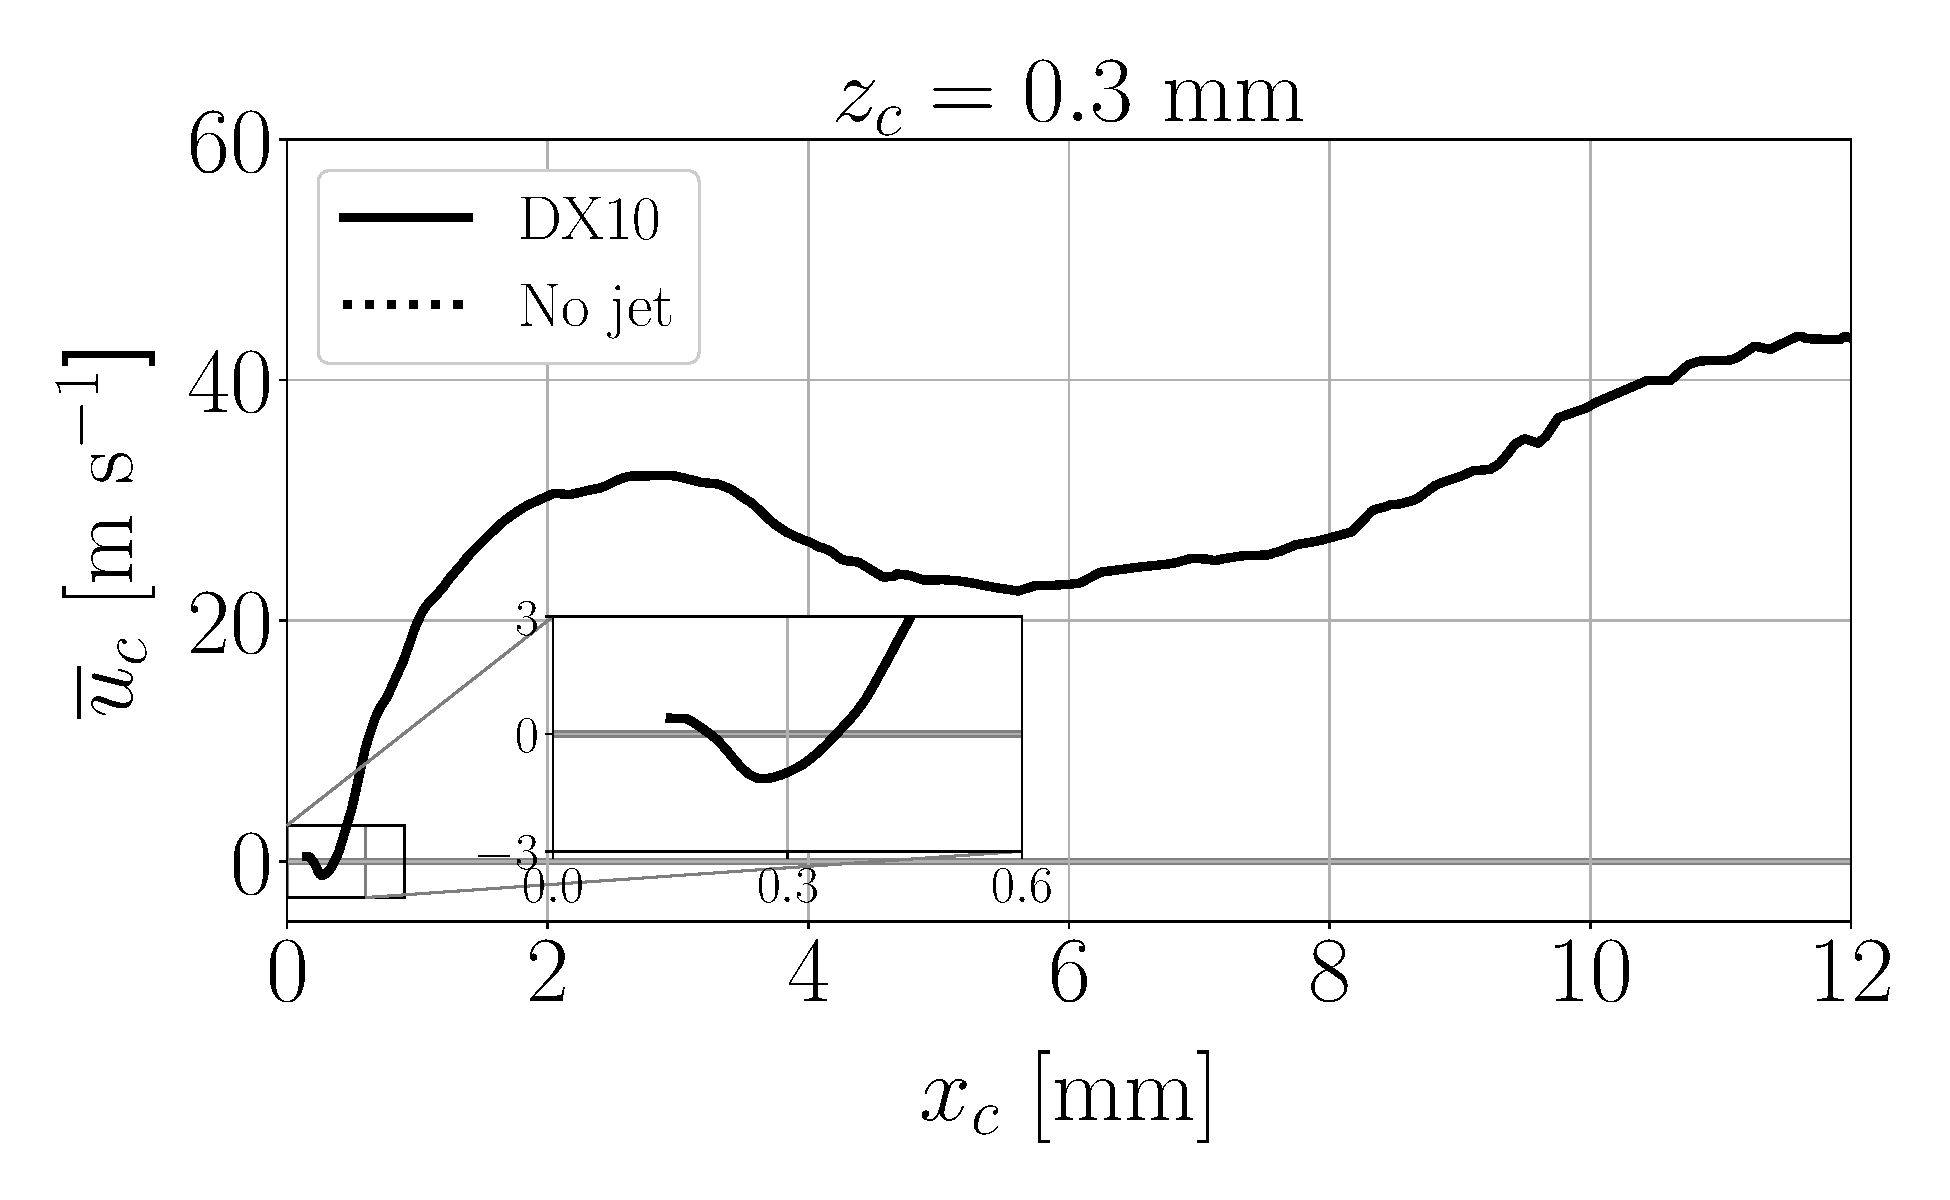
\includegraphics[scale=0.25]{./part3_applications/figures_ch9_lagrangian/gas_field_initial_conditions/line_y0_along_x_zlow}
   %\caption{}
   %\label{} 
\end{subfigure}
\hspace{0.4in}
\begin{subfigure}[b]{0.45\textwidth}
	\flushleft
   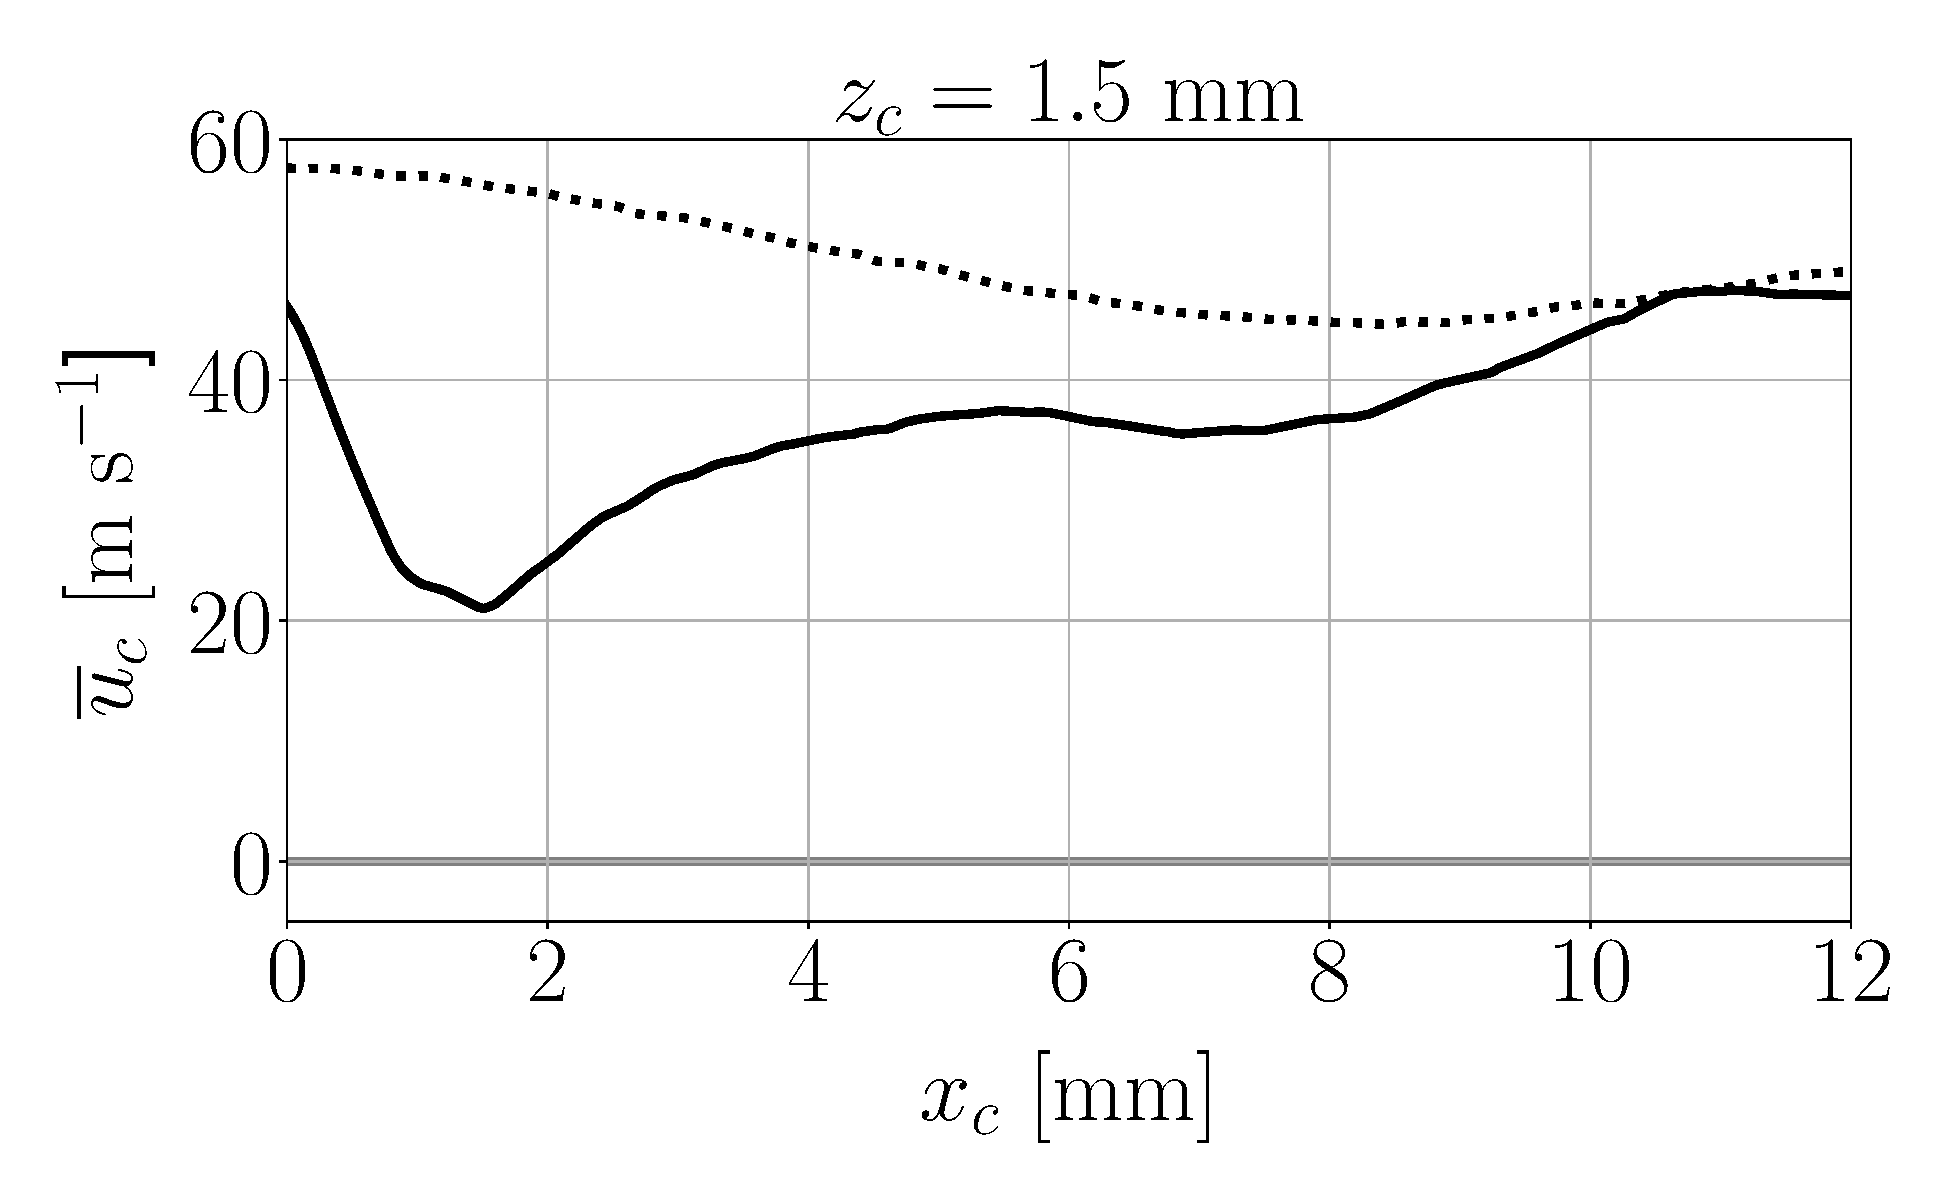
\includegraphics[scale=0.25]{./part3_applications/figures_ch9_lagrangian/gas_field_initial_conditions/line_y0_along_x_zhigh}
   %\caption{}
   %\label{}
\end{subfigure}
\caption{Mean axial velocity evolution along axial coordinate at locations $z_c = 0.3, 1.5$ mm at plane $y_c = 0$ (lines of Figure \ref{fig:BIMER_turbulent_structures_plane_y0})}
\label{fig:BIMER_LGS_lines_y0_along_x_ux_mean}
\end{figure}


\begin{figure}[ht]
\centering
   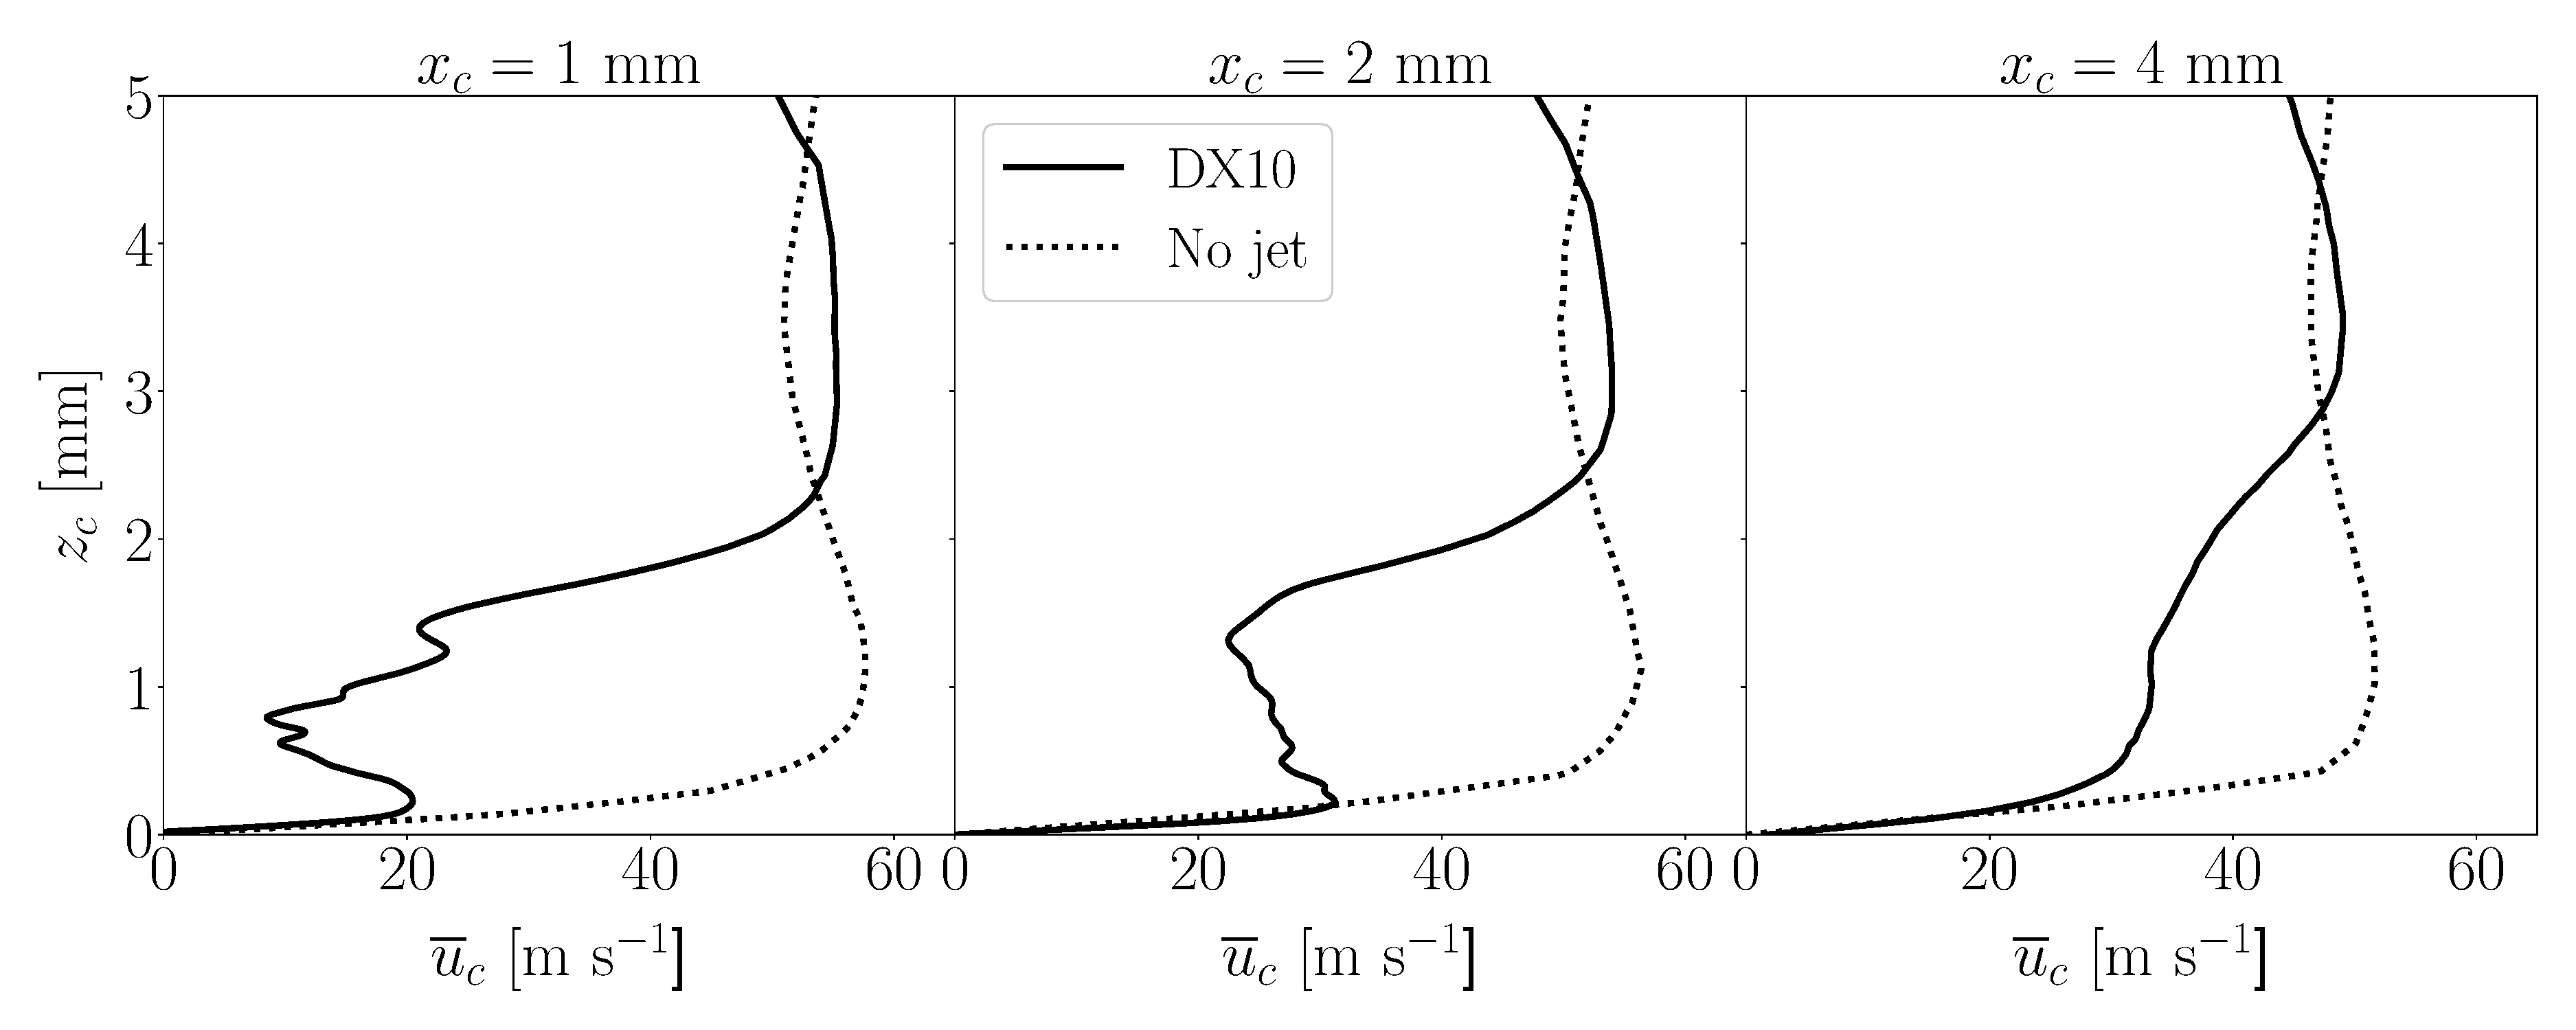
\includegraphics[scale=0.24]{./part3_applications/figures_ch9_lagrangian/gas_field_initial_conditions/lines_y0_along_z_ux_mean}
\caption{Mean axial velocity evolution along vertical coordinate at $x_c = 1, 2, 4$ mm locations of plane $y = 0$ (lines of Figure \ref{fig:BIMER_turbulent_structures_plane_y0})}
\label{fig:BIMER_LGS_lines_y0_along_z_ux_mean}
\end{figure}

The planes perpendicular to crossflow direction $x_c = 1.5, 3$ mm are also analyzed in Figure \ref{fig:BIMER_LGS_turbulent_structures_planes_x}.  As discussed in Chapter \ref{ch8:bimer_resolved_atomization}, the resolved simulations capture vortices which are not symmetrical along the $y_c = 0$ plane due to the presence of a swirl component in the gas. The unperturbed case shows actually strong single vortices which are caused by this swirl component, which demonstrates how swirl can affect the gaseous flow. ALM seems to affect the location and strength of the vortex at $x_c = 1.5$ mm, while i does not have a relevant effect on the one at $x_c = 3$ mm. In any case the actuator can retrieve the CVPs which are seen at the resolved simulation (at plane $x_c = 1.5$ mm, while further downstream a single vortex is captured). On the other hand, the ALM affects the gaseous field by creating a deceleration region, which at $x_c = 1.5$ mm also reflects the recirculation bubble. It is interesting to note that the recirculation bubble is does not reach plane $y_c = 0$, which agreeds with Figure \ref{fig:BIMER_LGS_turbulent_structures_plane_y0}  as recirculation in this plane attaches above this axial location. This indicates that the recirculation bubble is not symmetrical with respect to axis $y_c = 0$, which again is attributed to the presence of swirl. The fact that swirl has such a strong effect in this operating point (it is worth reminding that the swirl number is $S_w = 1$, as discussed in $\S$\ref{subsec:BIMER_ch7_sw_vortex_breakdown}) might then create a lateral force in the BIMER dense core which is not modelled by the ALM methodology proposed in this thesis. The velocity profiles along lines $z_c = 0.3, 1.5$ mm at the iso-$x_c$ planes from Figure \ref{fig:BIMER_LGS_lines_iso-x_along_y_ux_mean} show that effectively the ALM cannot capture the perturbations along the lateral directions: close to the wall the mean velocity is underestimated, and far from it it is overestimated for $y_c > 0$ mm. For a proper modelling of the gaseous phase perturbations within BIMER and other swirl injectors, ALM should then be extended to account for three-dimensional swirl effects. 


\begin{figure}[h]
\centering
   \includeinkscape[inkscapelatex=false,scale=0.30]{./part3_applications/figures_ch9_lagrangian/turbulent_structures/planes_x_ux_mean}
\caption[Mean axial velocity at planes $x_c = 1.5, 3$ mm for resolved DX10, gaseous unperturbed and gaseous ALM cases.]{Mean axial velocity at planes $x_c = 1.5, 3$ mm for resolved DX10, gaseous unperturbed and gaseous ALM cases. The vertical, white line corresponds to plane $y_c = 0$}
%{Mean axial velocity at planes $x = 5, 10$ mm. Black lines with arrows are in-plane mean streamlines. Instantaneous jets for each case are shown in transparent blue.}
\label{fig:BIMER_LGS_turbulent_structures_planes_x}
\end{figure}

The perturbations induced by ALM discussed previously have only been analyzed for the gaseous field at the surroundings of one liquid injection nozzle from the multipoint stage. Since in BIMER there are 10 points for this stage, perturbations also need to be added in those. This can be done by adding actuator body forces in the crossflow local coordinate systems at each point, and then transforming the coordinates and forces directions into the global coordinate system. In this way 10 actuators will be located, one per injection point, each one imposing forces with identical magnitude but different directions due to the different locations of the points around the take-off stage. An example of these multiple perturbations is shown in Figure \ref{fig:BIMER_ALM_revolution}, where the mean velocity magnitude in planes $y_c = 0$ at two different injection points are shown.

\clearpage


\begin{figure}[ht]
\centering
\begin{subfigure}[b]{1.0\textwidth}
	\centering
   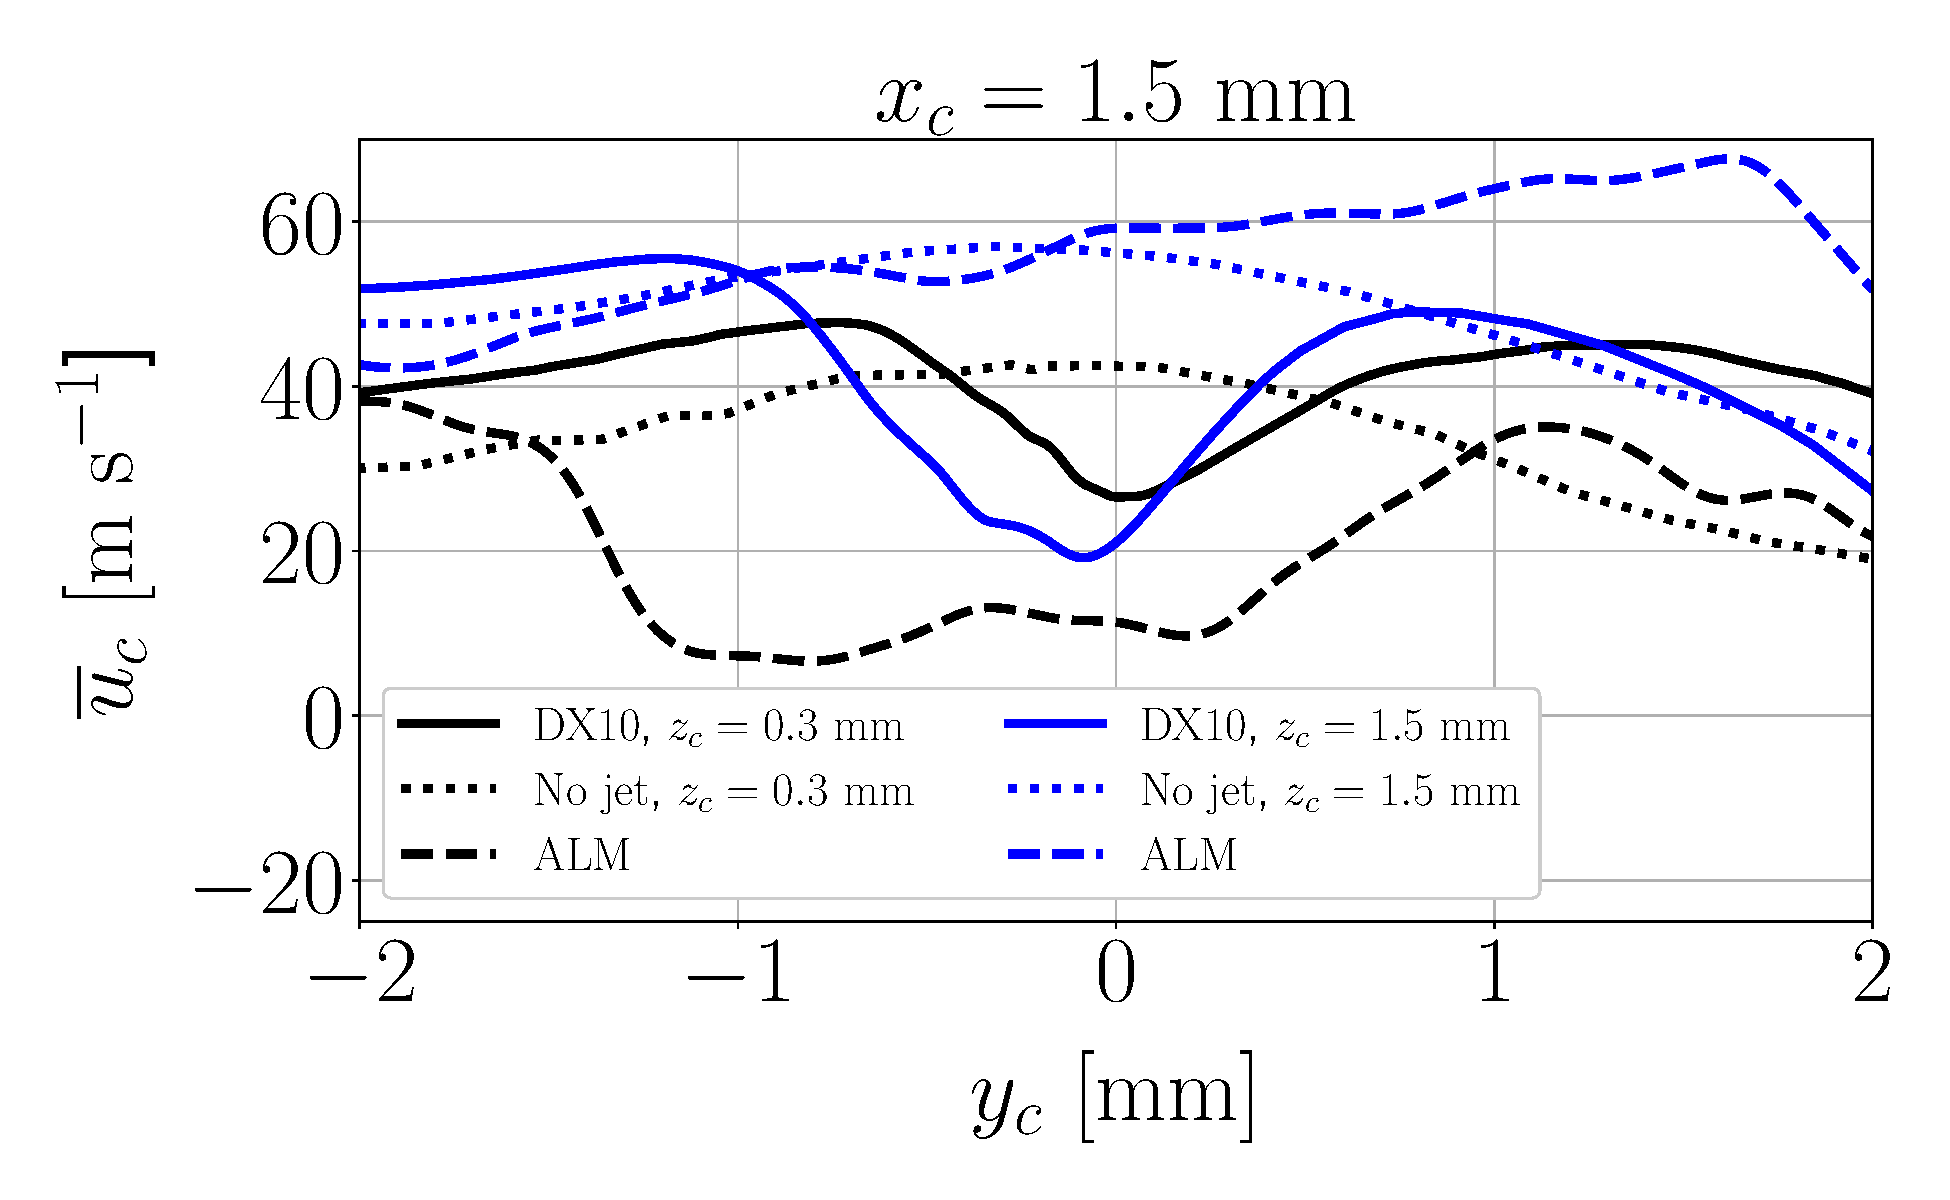
\includegraphics[scale=0.24]{./part3_applications/figures_ch9_lagrangian/gas_field_initial_conditions/lines_iso_x_along_y_plane_x01p5mm}
   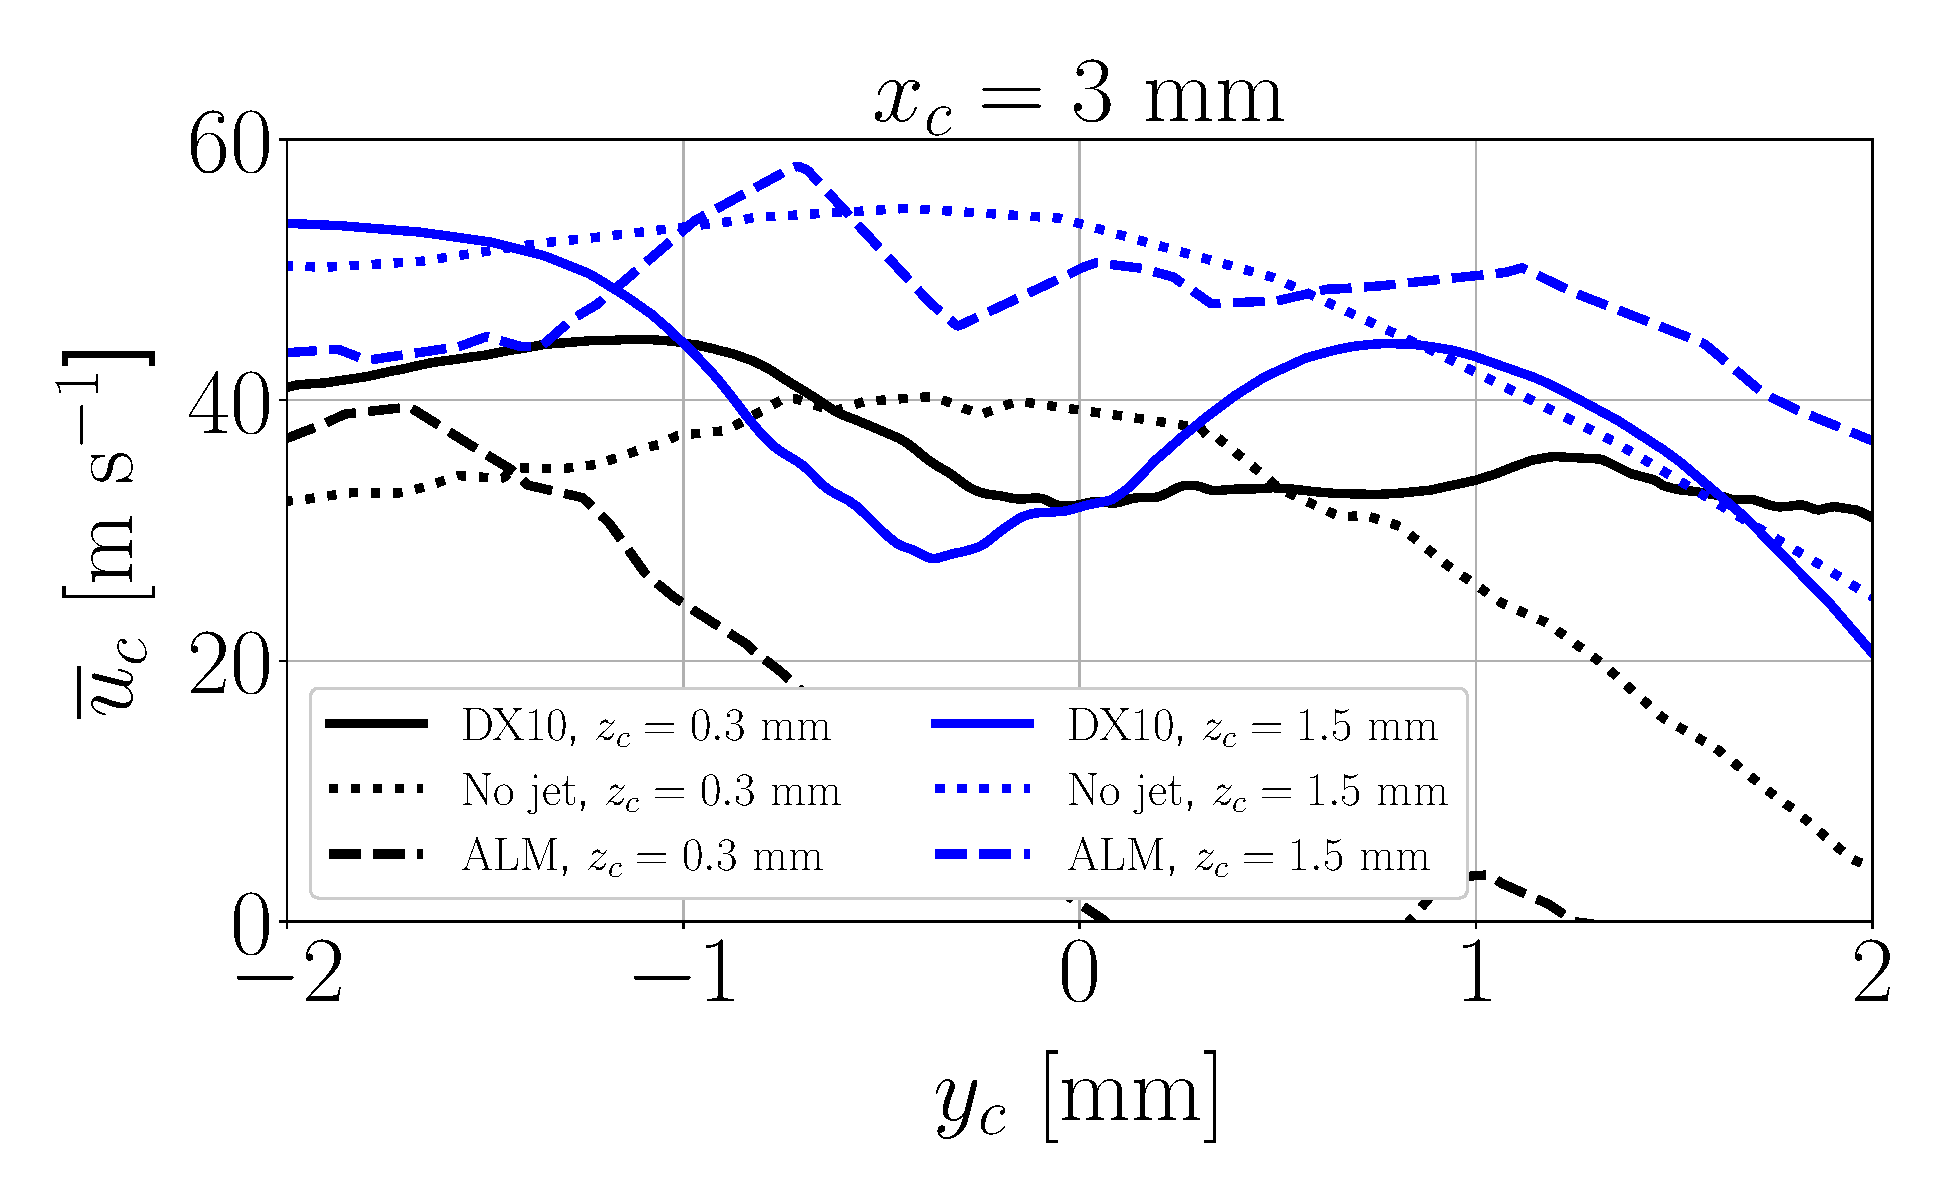
\includegraphics[scale=0.24]{./part3_applications/figures_ch9_lagrangian/gas_field_initial_conditions/lines_iso_x_along_y_plane_x03mm}
   %\vspace*{-0.1in}
\end{subfigure}
   \caption[{Mean axial velocity evolution along lateral coordinate at $z_c$ lines of Figure \ref{fig:BIMER_turbulent_structures_planes_z}}]{Mean axial velocity evolution along lateral coordinate at $z_c$ lines of Figure \ref{fig:BIMER_turbulent_structures_planes_z}. Dotted circles englobe gaseous vortical structures}
\label{fig:BIMER_LGS_lines_iso-x_along_y_ux_mean}
% OJO: ALM ones belong to restart_03 sol 08
\end{figure}


\begin{figure}[ht]
\centering
\begin{subfigure}[b]{1.0\textwidth}
	\centering
   
\includegraphics[scale=0.18]{./part3_applications/figures_ch9_lagrangian/turbulent_structures/ALM_revolution}
   %\vspace*{-0.1in}
\end{subfigure}
   \caption{Application of the ALM model to two adjacent injectos in BIMER}
\label{fig:BIMER_ALM_revolution}
\end{figure}

\section{Simulations and results}

Three dispersed-phase simulations are performed for the BIMER configuration. All of them use the same boundary conditions for the liquid phases in the take-off (SLI model) and the pilot (LISA model) stages. They differ in the inclusion of the perturbation effect in the gaseous phase through ALM and the consideration of evaporation. For the simulation with evaporation, the full domain is preheated to $T_g = 433$ K as in the experiments, and droplets are then injected at a temperature $T_l = 293 $ K.  The computations performed are summarized in Table \ref{tab:BIMER_dispersed_phase_simulations_performed}, where a total of three simulations are reported. A baseline simulation is performed without neither ALM nor evaporation. Then, both ALM and evaporation contributions are studied separately in two distinct simulations.

\begin{table}[!h]
\centering
\caption{Dispersed-phase simulations performed for BIMER}
\begin{tabular}{ccc}
\thickhline
\textbf{Case} & \textbf{ALM} & \textbf{Evaporation} \\
\thickhline
Baseline & No & No \\
ALM & Yes & No \\
Evap & No & Yes \\%\textcolor{blue}{Yes} \\
\thickhline
\end{tabular}
\label{tab:BIMER_dispersed_phase_simulations_performed}
\end{table}


\subsubsection*{Characteristic liquid times}

As in the resolved atomization simulations of one multipoint injector, characteristic liquid times can be defined for the liquid phase in the dispersed-phase computations. The interest here is to relate the physical simulation time to a characteristic time scale related to the magnitudes to be studied. In this case, these magnitudes are the SMD and droplets velocities in the spatial region downstream the combustion chamber where experimental PDA results have been obtained (Figure \ref{fig:maps_BIMER_renaud_expe_results}). Since this region spans up to a downstream coordinate $x = 35$ mm, droplets characteristics time will be estimated as the time in which the first particle reaches this axial location: $\tau_{\mathrm{dr}_{x=35\mathrm{mm}}}$. Therefore, the dimensionless simulated time $t^{\prime}$ is defined according to Eq. (\ref{eq:t_prime_BIMER_LGS}):

\begin{equation}
\label{eq:t_prime_BIMER_LGS}
t^{\prime} = t / \tau_{\mathrm{dr}_{x=35\mathrm{mm}}}
\end{equation}


Table \ref{tab:BIMER_dispersed_phase_characteristic_times}.  summarized the characteristic times obtained in the simulations performed. As observed in this table, the characteristic times chosen are of the order of the gaseous swirl time scale $\tau_\mathrm{swirl}$ for this operating point (Table \ref{tab:gaseous_field_timescales}) while they differ of one order of magnitude with respect to the liquid characteristic times of the resolved atomization simulations (see Tables \ref{tab:BIMER_SPS_characteristic times} and \ref{tab:BIMER_SPS_characteristic_droplet_sampling_times}).  This shows again (this was also demonstrated in the lagrangian simulations of Chapter \ref{ch6:jicf_lgs_simulations}) how the dispersed phase computations allow to simulate more physical times and obtain converged spray fields with less computational time than the resolved atomization simulations. 


\begin{table}[!h]
\centering
\caption{Characteristic times for droplets to reach location $x = 35$ mm in the pilot and take-off stages }
\begin{tabular}{ccc}
\thickhline
\textbf{Case} & $\tau_{\mathrm{dr}_\mathrm{pilot}}$ [ms] & $\tau_{\mathrm{dr}_\mathrm{takeoff}}$ [ms] \\
\thickhline
Baseline & 1.65 & 2.45 \\  % restart_01, it. 330 ; restart_01, it. XX
ALM & 1.52 & 2.32 \\ % restart_02, it. 143
Evap & 1.48 & 2.25 \\ % restart_01, it. 295
\thickhline
\end{tabular}
\label{tab:BIMER_dispersed_phase_characteristic_times}
\end{table}





\subsection{Lagrangian field establishment}

The three simulations summarized in Table \ref{tab:BIMER_dispersed_phase_simulations_performed} are performed with identical liquid dispersed-phase injection boundary conditions and with their corresponding boundary conditions for the gaseous phase. In all cases, liquid has been injected into a established single-phase gaseous solution which was previously run for $2 \tau_\mathrm{conv}$, being $\tau_\mathrm{conv} = 37.6$ ms the convection time scale described in Chapter \ref{ch7:bimer_test_bench_and_aero}. Running for such time corresponds to $\sim 8 \tau_\mathrm{swirl}$, which ensures a established gaseous field within the injector for all simulations.

The establishment of the dispersed-phase liquid field is shown in Figure \ref{fig:BIMER_LGS_spray_establishment} for the Baseline case. Time has been expressed non-dimensionless with Eq. (\ref{eq:t_dimensionless_with_tau_in}), where the inertia timescale $\tau_\mathrm{in}$ from Table \ref{tab:BIMER_SPS_characteristic times} has been used. The figures show droplets being injected through all the SLI located at the vicinity of each multi-point hole and through the pilot stage. Particles delivered through the take-off stage have different sizes due to the poly-disperse nature of SLI, which injects droplets from 20 to 40 $\mu$m of diameter (see Figure \ref{fig:injectors_sli_BIMER_DX10_xD06p67}),. These particles travel within the injector in the azimuthal direction, transported by the air swirl, and eventually are transported through the diffuser towards the combustion chamber. Simultaneously, the pilot stage introduces a mono-disperse spray with a imposed size of 15 $\mu$m with a hollow-cone type injection. The hollow cone shows then an oscillatory behaviour due to the interaction among the rotation of the air that arrives from the pilot swirler (schematically shown in Figure \ref{fig:BIMER_swirler}) and an azimuthal component imposed to the particles by the LISA model (Eq. \ref{eq:LISA_model_u_theta}). Pilot particles are then directly transported downstream the diffuser and arrive in the plenum before the droplets injected by SLI, as reflected by the characteristic times of Figure \ref{tab:BIMER_dispersed_phase_characteristic_times}.

\clearpage

\begin{figure}[h!]
	\centering	\includeinkscape[inkscapelatex=false,scale=0.6]{./part3_applications/figures_ch9_lagrangian/LGS_establishment_baseline_case}
	\caption[Several instants of liquid fuel injection through both pilot and take-off stages for baseline case]{Several instants of liquid fuel injection through both pilot and take-off stages for baseline case. Droplets are scaled by 10 times their diameter for visualization purposes}	\label{fig:BIMER_LGS_spray_establishment}
\end{figure}


Figure \ref{fig:BIMER_LGS_spray_established_jets}. shows a lateral view of established sprays for the three simulations performed. The experimental region for the $SMD$ and axial velocity maps is outlined by the black rectangle. The first row shows the full spray: once the spray is established, particles from both pilot and multipoint stages are found in the diffuser and further downstream. The baseline and ALM cases do not show any significant differences. The evaporation simulation, on the other hand, reveals that smaller particles are found already within the diffuser, indicating that mass transfer from the SLI particles starts to take place prior being introduced to the diffuser. Overall, all cases show a good topology of the particles field within the injector and at the upper part of the plenum, similar to other particles fields performed in other multipoint configurations with dispersed-phase simulations \citepColor[jaegle_eulerian_2011]. 

Particles within a slab of 1 mm thickness centered at plane $z = 0$ are also shown in Figure \ref{fig:BIMER_LGS_spray_established_jets}..  The full spray and the contribution of each separate phase are shown. The pilot particles are shown to open with an angle corresponding to the imposed one of $30~\deg$ with the LISA model. Such particles show a high concentration within the slab close to the injection point and then show empty pockets further downstream: these particles are firstly injected through the pilot at a low axial velocity and a rotational component, then they are convected and exchange momentum with the swirl, relaxing towards the gaseous velocity which also has both an axial and an azimuthal component. Therefore, the observed pockets are caused by particles leaving the slab due to the rotational movement; these particles will later enter the slab further downstream, as visualized in the figure. The multipoint particles enter the diffuser and the vicinity of the walls, with a high number of particles filming along the diffuser walls in all cases. There are no particles injected through the multipoint found within the central region of the spray downstream the diffuser, as it is shown later through the maps in Figure \ref{fig:comparison_pilot_takeoff_maps_BIMER_lgs}.


\begin{figure}[h!]
	\centering	\includeinkscape[inkscapelatex=false,scale=0.5]{./part3_applications/figures_ch9_lagrangian/LGS_comparison_case}
	\caption[Instantaneous views with a established spray for the three disperse-phase computations]{Instantaneous views with a established spray for the three disperse-phase computations. In the first row the full lagrangian field is shown, while the second row displays the spray contained within a slab of 1 mm thickness centered at the center of the injector. The third and fourth rows show the droplets from the pilot and take-off stages respectively, contained in the 1 mm thick slab.}	
	\label{fig:BIMER_LGS_spray_established_jets}
\end{figure}



\subsection{Qualitative results and experimental comparison}

Simulations can be compared with experiments by sampling the lagrangian droplets that cross the enclosed region depicted in Figure \ref{fig:BIMER_LGS_spray_establishment}, which corresponds to the spatial area where the experimental results shown in Figure \ref{fig:maps_BIMER_renaud_expe_results} were obtained. SMD and droplets axial velocities results are shown in Figure \ref{fig:validation_BIMER_lgs}. In general, the computations capture the topology of the fields accurately and show symmetry with respect to axis $y = 0$. The effect of the evaporation is clearly seen by the lower values of SMD found with respect to the other computations, matching better the experimental values. Numerical size maps show a central region with low SMDs produced by the pilot stage, which for the baseline and ALM cases shows larger sizes than in the experiments and the opposite for the evaporation simulation. The experiments show a pocket of empty droplets with a circular shape with center at $x = 10, y = 0$ mm and a radius of $\sim 20$ mm that is not present in the simulations, since these show droplets produced by the hollow cone, and two regions of local high SMDs at $y = \pm 25$ mm that are quantitatively capture by the simulations, even if their size slightly underestimated and the axial extension of this area is overestimated in the computations. The opening angle of the spray is properly captured by the simulations, although this angle is determined by the presence of the diffuser as Figure \ref{fig:BIMER_LGS_spray_establishment} shows droplets attaching and filming along the diffuser walls. Diameters at the outer part of the spray show larger values than at the center as in the experiments, yet their magnitude is generally overestimated with respect to those. This outer part, also captured by the experiments, is characterized by a gradient of SMD from lower to larger values along the vertical direction. The computations predict its beginning closer to the spray center than in the experiments, and overestimate the SMD values at the edges for both the baseline and ALM cases. The evaporation case shows good experimental match for SMD values in this region, except for the outer part for $y > 0$. Figure \ref{fig:comparison_pilot_takeoff_maps_BIMER_lgs} shows that ...

show a transition from lower SMDs in the region closer to the pilot

The evaporation case 



\begin{figure}[h!]
\centering
\begin{subfigure}[b]{1.0\textwidth}
	\centering 
	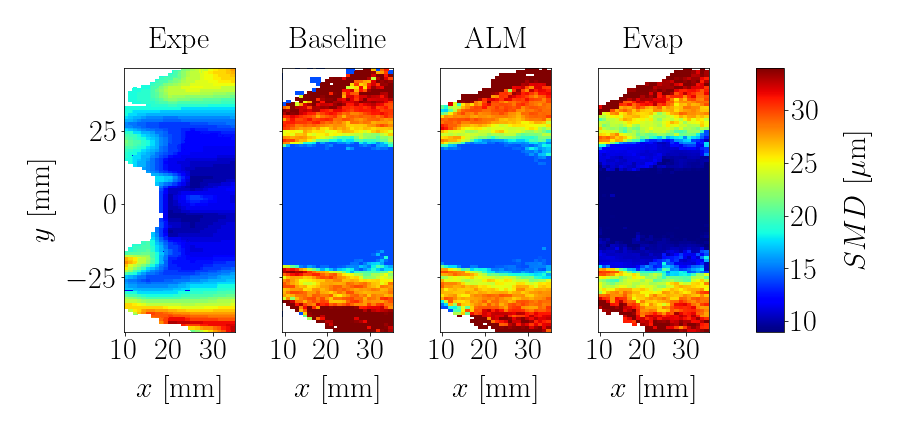
\includegraphics[scale=0.7]{./part3_applications/figures_ch9_lagrangian/simus_expe_validation/subplots_maps_SMD.png}
   \caption{SMD maps}
   %\label{fig:validation_qualitative_u_mean} 
\end{subfigure}

\vspace*{0.1in}

\begin{subfigure}[b]{1.0\textwidth}
	\centering
	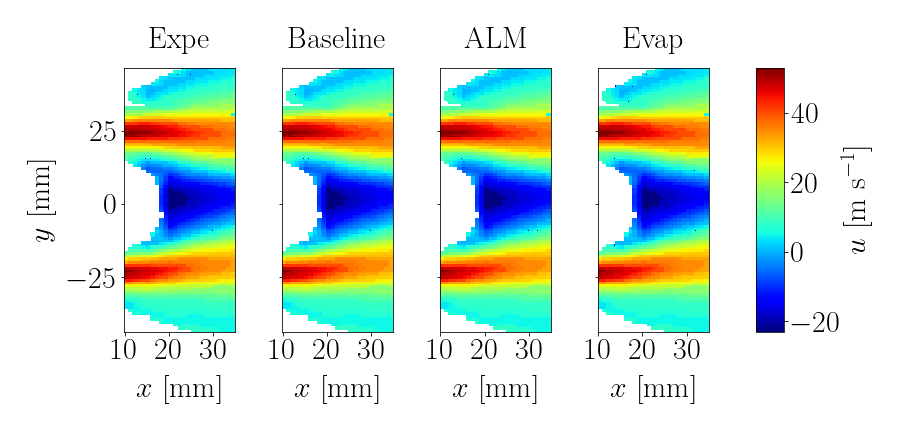
\includegraphics[scale=0.7]{./part3_applications/figures_ch9_lagrangian/simus_expe_validation/subplots_maps_axial_velocity.png}
   \caption{Mean axial velocity maps}
\end{subfigure}
%
%\vspace*{0.1in}
%
%\begin{subfigure}[b]{1.0\textwidth}
%	\centering
%	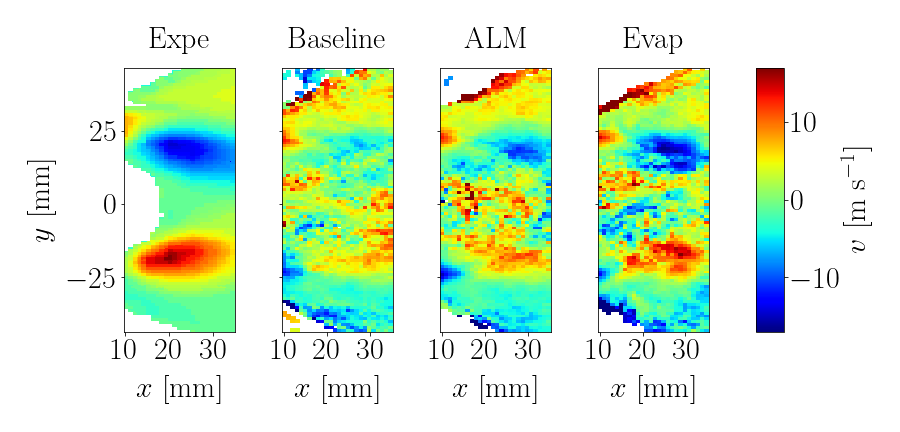
\includegraphics[scale=0.4]{./part3_applications/figures_ch9_lagrangian/simus_expe_validation/subplots_maps_vertical_velocity.png}
%   \caption{Mean vertical velocity maps}
%   %\label{fig:validation_qualitative_v_mean} 
%\end{subfigure}
\caption[Qualitative experimental validation]{Qualitative experimental validation in the region enclosed in Figure \ref{fig:BIMER_LGS_spray_establishment}. SMD and mean velocity fields from experiments by \citeColor[renaud_high-speed_2015] and the three simulations performed}
\label{fig:validation_BIMER_lgs}
\end{figure}

\clearpage



\begin{figure}[h!]
\centering
\begin{subfigure}[b]{1.0\textwidth}
	\centering 
	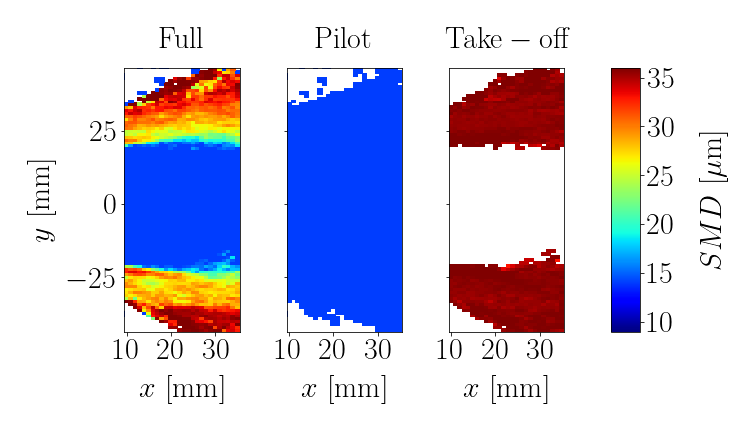
\includegraphics[scale=0.5]{./part3_applications/figures_ch9_lagrangian/simus_pilot_takeoff_comparison/baseline_SMD.png}
\hspace*{0.1in}
   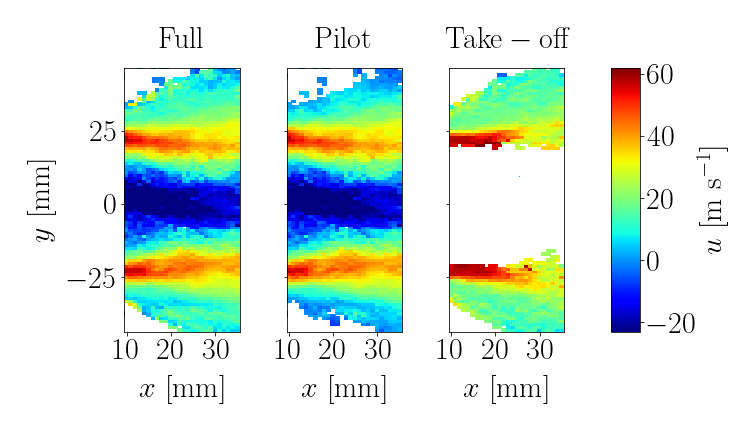
\includegraphics[scale=0.5]{./part3_applications/figures_ch9_lagrangian/simus_pilot_takeoff_comparison/baseline_u_axial.png}
   \caption{Baseline case}
   %\label{fig:validation_qualitative_u_mean} 
\end{subfigure}

\vspace*{0.1in}

\begin{subfigure}[b]{1.0\textwidth}
	\centering
	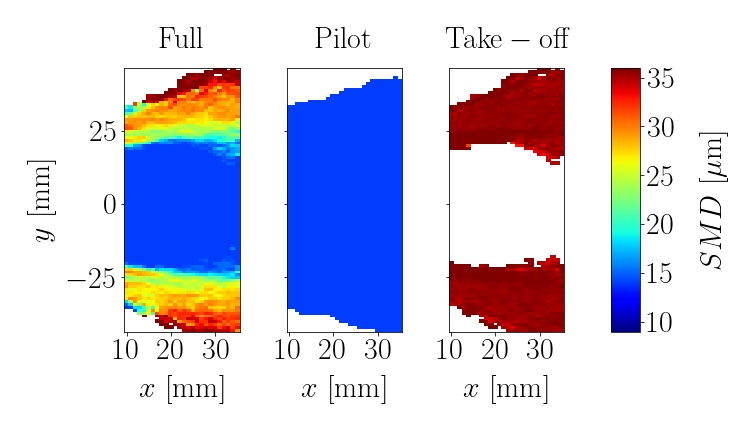
\includegraphics[scale=0.5]{./part3_applications/figures_ch9_lagrangian/simus_pilot_takeoff_comparison/ALM_SMD.png}
\hspace*{0.1in}
   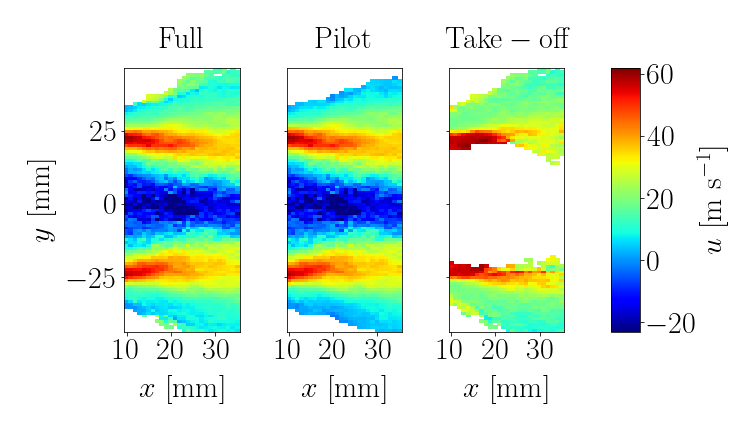
\includegraphics[scale=0.5]{./part3_applications/figures_ch9_lagrangian/simus_pilot_takeoff_comparison/ALM_u_axial.png}
   \caption{ALM case}
\end{subfigure}

\vspace*{0.1in}

\begin{subfigure}[b]{1.0\textwidth}
	\centering
	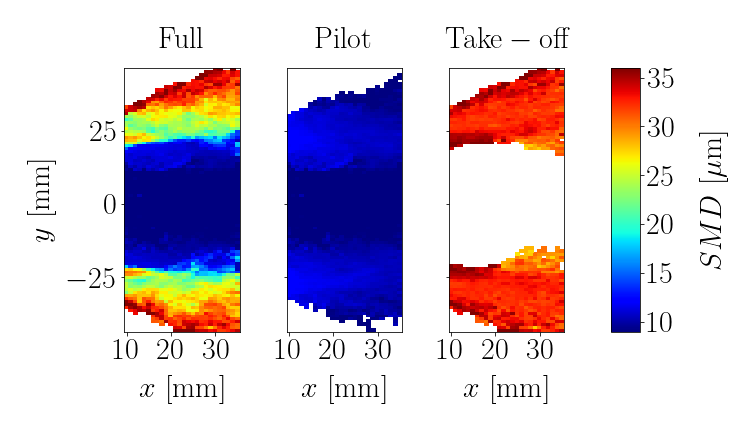
\includegraphics[scale=0.5]{./part3_applications/figures_ch9_lagrangian/simus_pilot_takeoff_comparison/evap_SMD.png}
\hspace*{0.1in}
   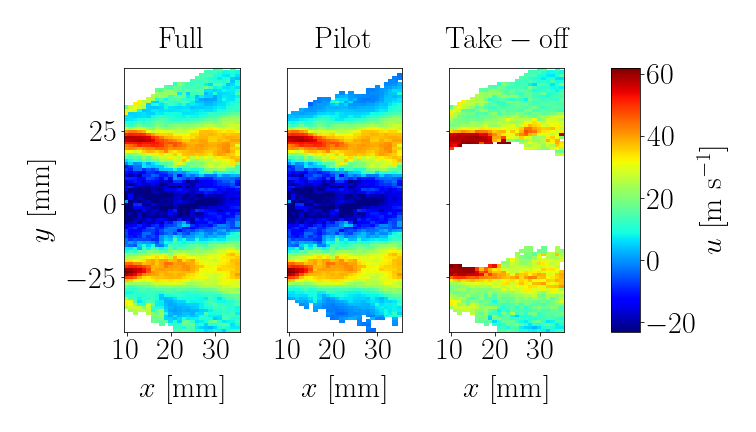
\includegraphics[scale=0.5]{./part3_applications/figures_ch9_lagrangian/simus_pilot_takeoff_comparison/evap_u_axial.png}
   \caption{Evap case}
\end{subfigure}
\caption[Comparison of pilot and take-off stages to the resulting
spray ]{Comparison of pilot and take-off stages to the resulting
spray in the experimental validation region outlined in Figure \ref{fig:BIMER_LGS_spray_establishment}}
\label{fig:comparison_pilot_takeoff_maps_BIMER_lgs}
\end{figure}

The global SMD of the droplet contained in the regions shown in Figure \ref{fig:validation_BIMER_lgs} are shown in Table \ref{tab:BIMER_dispersed_phase_characteristic_times}.  The first SMD shown corresponds to the full case (pilot + take-off sprays), while the global SMD for each separate phase in the computations is also reported.  The error with respect to the experiments $\varepsilon_{SMD}$ has been calculated with Eq. (\ref{eq:error_expe_SMD_LGS_simus}), with $SMD_\mathrm{expe} = 16.58~\mu$m. Only the deviation in SMD for the full spray can be quantified, since from the experimental results the SMDs for each separate phase cannot be obtained. The results show that the baseline and ALM cases provide similar values larger than experiments, with errors of the order of 30 $\%$. The SMDs for these cases are practically identical for the full, pilot and take-off sprays. Indeed, the pilot spray for these cases yields the value prescribed for the injected droplets of $15~\mu$m since these droplets do not change their size due to the absence of secondary atomization and evaporation. This indicates that, in BIMER, the actuator model tested has not a significant influence in the spray, even if it perturbs the gaseous phase around the injection nozzles of the take-off stage. Such lack of influence is due to the inexisting secondary atomization in BIMER, as the results from Chapter \ref{ch6:jicf_lgs_simulations} showed that the ALM had a strong influence on the atomization of droplets in the dispersed-phase. 

\clearpage

More relevant results are obtained when including evaporation. As Table \ref{tab:BIMER_dispersed_phase_characteristic_times} shows, addition of evaporation reduces the pilot SMD from 15 to 9.41 $\mu$m, and the corresponding one for the take-off stage from 35.81 to 32.67 $\mu$m. In consequence, the global SMD obtained is 17.53 $\mu$m which supposses an error of $5.73~\%$, showing a very good experimental agreement. Plugging evaporation physics into the dispersed-phase simulation contributed then to improve the results of the simulations, as shown by the maps and SMD values.



\begin{table}[!h]
\centering
\caption{SMDs obtained compared to experimental one}
\begin{tabular}{ccccc}
\thickhline
\textbf{Case} & $SMD$ [$\mu$m] & $\varepsilon_{SMD}~\left[\% \right]$ & $SMD_\mathrm{pilot}$ [$\mu$m] & $SMD_\mathrm{takeoff}$ [$\mu$m]   \\
\thickhline
Experiments & 16.58 & - & - & - \\
Baseline & 21.41 & 29.13 &15.00 & 35.81 \\
ALM & 21.17 & 27.68 & 15.00 & 35.71 \\
Evap & 17.53 & 5.73 & 9.41 & 32.67 \\ 
\thickhline
\end{tabular}
\label{tab:BIMER_dispersed_phase_characteristic_times}
\end{table}


The effect of evaporation in both pilot and take-off phases separately can be seen by looking at the droplets histograms obtained within the experimental comparison region for the baseline and evaporation cases shown in Figure \ref{fig:LGS_BIMER_droplets_histograms}. The take-off and pilot stages can be directly distinguished by the different in the range of droplets sizes obtained: the largest pilot droplets have diameters of $15~\mu$m, while the smallest particles produced by the take-off are slightly below $30~\mu$m. The spray for the baseline case shows a single diameter for pilot at $15~\mu$m, and a distribution for the take-off ranging from $\sim 35$ to $\sim 42~\mu$. Adding evaporation shifts each histogram to the left. The pilot distribution shows then a polydisperse spray negatively skewed, with the largest diameters at $14~\mu$ and the smallest ones close at $1~\mu$, while the take-off stage moves towards a lognormal-like distribution but without large differences among density values.




\begin{figure}[ht]
   \centering
   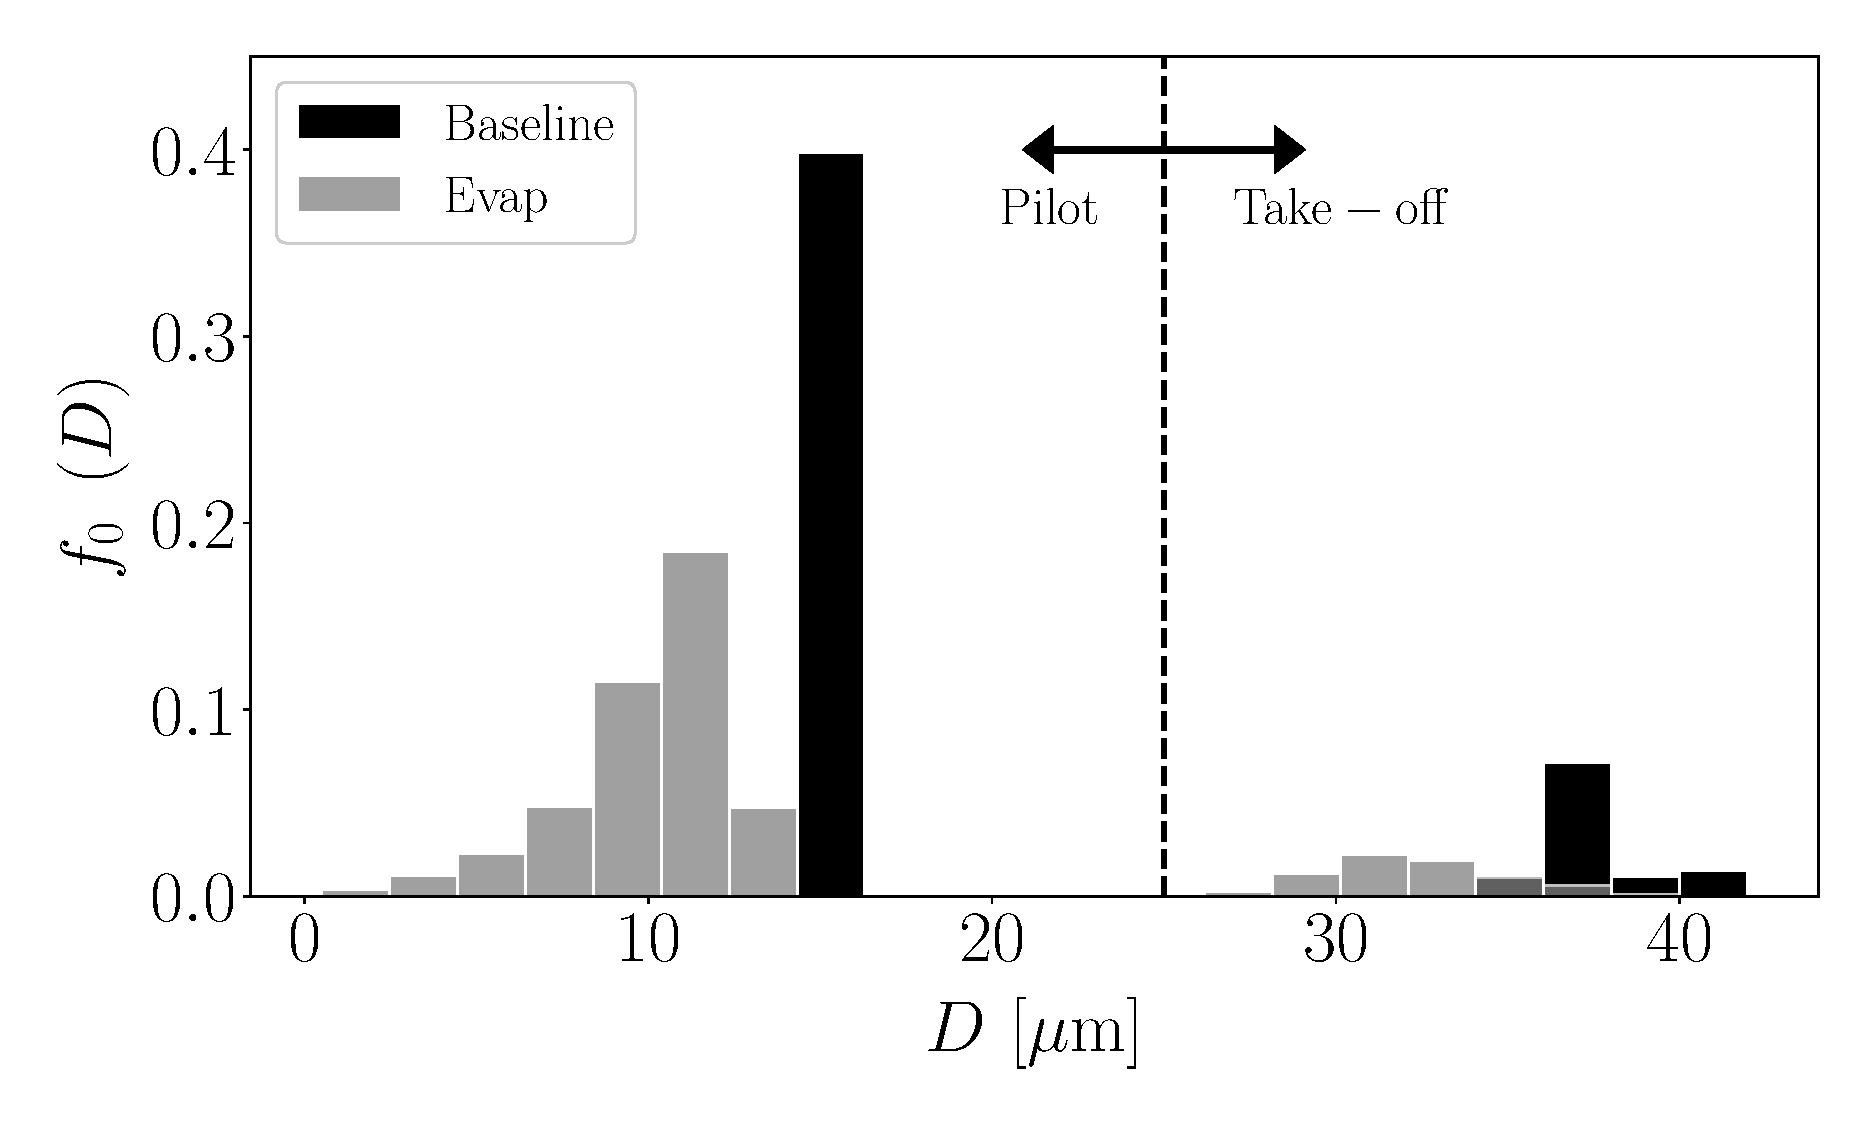
\includegraphics[scale=0.4]{./part3_applications/figures_ch9_lagrangian/droplets_histograms}
   \caption{Cost savings in SLI development by refining grid resolution}
   \label{fig:LGS_BIMER_droplets_histograms}
\end{figure}

In conclusion, the addition of evaporation, which can be accounted for in dispersed-phase simulations, is necessary to capture accurately the dispersed-phase within the plenum in BIMER due to the high ambient temperature. It is not known a priori how evaporation would influence the droplets sizes in the resolved atomization simulations: if it had a relevant effect, this could affect the SLIs obtained and the subsequent results of the dispersed-phase simulations. Nevertheless, the time-scales of the droplets convection, in Tables \ref{tab:BIMER_SPS_characteristic_droplet_sampling_times} and \ref{tab:BIMER_dispersed_phase_characteristic_times} for the resolved and dispersed-phase simulations respectively, show that a resolved droplet takes $0.354$ ms to reach the sampling plane located 2 mm  away from the take-off injection nozzle, and a lagrangian droplet needs 2.25 ms (in the evaporation case) to reach the axial location $x = 35$ mm in the plenum. Therefore, in the dispersed case droplets travel for more than $35$ mm (this is only the axial location, not accounting for the path followed by the droplet within the inject due to the air swirl) after being injected and see a reduction in SMD from 35.81 to 32.67, while in the resolved simulations the droplet travels only for less than 2 mm (since actually the droplet is first atomized from the dense core, which could hardly evaporate due to its large volume and low surface-to-volume ratio). Therefore, it is expected that evaporation would not have a large influence on the SLIs from the resolved atomization simulations due to the locations of the sampling planes close to injection, giving robustness to the results presented in this chapter.

%\section{Computational performances}
%
%In 

%\section{Computational performances}

\section{Conclusions}


This chapter has shown the application of SLI to initialize the dispersed liquid phase in the academic multipoint injector BIMER. The methodology has been applied to the take-off stage by using the SLI constructued from the resolved atomization simulations of Chapter \ref{ch8:bimer_resolved_atomization}. The SLI obtained from one injection hole has been extrapolated to the rest of the multipoint to initialize the liquid phase in all the take-off stage. This has been possible thanks to the symmetry of the multipoint injector. The pilot stage, which produces a hollow cone-type injection, has been approximated with the LISA 
model. For the gaseous phase, the ALM methodology has been applied to model the perturbation of the BIMER dense core in the aerodynamic field. As in the SLI, the perturbation effect has been studied in the resolved simulations for one injection hole and then extrapolated to the rest of injectors in the dispersed-phase simulation. To study the influence of the ALM, one simulation has been without perturbing the gaseous phase at the vicinity of the injectors by taking as initial conditions the simulation from Chapter \ref{ch7:bimer_test_bench_and_aero}. \hl{Additionally, evaporation has also been included in a third simulation to better replicate the multiphysics conditions found within these injectors, since ambient temperature in the operating point studied is high enough for evaporation to take place.}

\hl{We also need to specify that the initial conditions for ALM extracted from the resolved simulations are not so useful to replicate the actual perturbation effect of the dense core, as in the simulations from Chapter \textbf{XX}. These parameters must then be tuned in order to obtain a better match for the perturbation effect. In this work, this tuning has been performed by hand: a more elegant way to obtain a more reliable ALM could be through a multi-parameter optimization process to find an optimal actuator from the initial conditions through an iterative process (\textbf{ref?}). Furthermore, including transient effects in the actuator (such as variable end point coordinates and forces) through a spectral strategy could also help to improve the performances of the ALM.}

\hl{Results have shown ....}

Further work is required in order to accurately match the experimental results. Nevertheless, this chapter has shown the capability of SLI to initialise the spray in dispersed-phase simulations from more realistic, industrial-type multi-staged burners, and its ability to add multiphysical phenomena such as evaporation. Next steps include adding a flame kernel to ignite the reactive gas-fuel mixture and simulate combustion.


